Evaluation of the vocabulary list generation approaches is challenging:
The accuracy of the approaches is evaluated by evaluating the efficiency of the vocabulary lists.
We have described in detail our approach to vocabulary efficiency evaluation in Section \ref{sec:experimental-setup-with-ai}, which involves running an AI model on a context-specific corpus with a given vocabulary, where the vocabulary is given by taking the first n $k$ words from the vocabulary list in question.
However, this approach is very similar to our approach for list generation, which involves analyzing AI interaction of AI models with corpora through the use of XAI methods.
Therefore, it is natural to assume that our evaluation approach is biased towards the lists stemming from our list generation approach.
This concern is especially pertinent as it has been shown that AI models do not reliably respond comparably to humans when the inputs to NLP tasks are perturbed \cite{tjuatjaLLMsExhibitHumanlike2024}.

To the best of our knowledge, there has not yet been a proposed evaluation metric for vocabulary lists that can be done automatically and which outputs a simple numeric result.
For this reason, in addition to our own evaluation approach utilizing AI models, we take some sample vocabulary lists, use our evaluation approach, and check whether the results align with human intuition.

For this reason, our evaluation is not only concerned with analyzing statistics of measured efficiency, but also with whether the calculated efficiency values are reliable.
The questions examined in this chapter can be summed up as:
\begin{enumerate}
	\item Does the efficiency evaluation of our list correspond with human intuition?
	\item Does our generation approach outperform frequency-based approaches?
	\item What are the upsides/downsides of each list generation approach (accuracy, speed, free choice of corpora)?
	\item How can the various approaches be combined to supplement each other's weaknesses?
\end{enumerate}

\todo{Add section references when chapter structure is fixed}
The following sections first describe the (numeric) metrics used in the evaluation.
We then introduce several baselines against which we compare our list generation approach.
The baselines include both publicly available vocabulary lists from online language learning tools, and existing list compilation methods introduced in Section \ref{sec:frequency-based-list-generation-methods} in connection with the corpora used for our own lists for a more direct comparison.

We then present the results of the evaluation, as well as discuss their implications.

\section{Evaluation Measures}

The various utility extraction approaches produce ranked lists as outputs.
To compare these, we employ both quantitative and qualitative comparison approaches, described in the following sections.



\subsection{NLP Task Performance}
Our primary metric for evaluating a vocabulary list's efficiency is the approach explained in Section \ref{sec:experimental-setup-with-ai}:
We let an AI model perform an NLP task with a vocabulary $V_{l, k}$, consisting of the first $k$ elements of the list $l$.
The limited vocabulary is simulated by removing words outside the vocabulary from the inputs to the model.
For illustration, consider the example sentence:

\begin{quote}
	\textit{Abraham Lincoln faced enmity in 1863.}
\end{quote}

If our vocabulary consists only of the word \textit{enmity}, this sentence becomes:

\begin{quote}
	\textit{Abraham Lincoln enmity 1863.}
\end{quote}

Since \textit{Abraham Lincoln} is recognized as a named entity, we leave it in the input, even though it is not part of the vocabulary.
Non-alphabetic tokens, such as numbers and punctuation, are also left in the input.


We start the evaluation of every vocabulary list with a vocabulary size of 0, letting the model run on inputs where only named entities and non-alphabetic are left.
The score for the entire corpus is calculated by taking the arithmetic mean of the scores of individual lines.
This allows us to see the "utility" of the named entities on their own, putting into comparison the following performance scores in our evaluation.
After this, we set the vocabulary size to 10 words, and run the AI models with the resulting vocabulary $V_{l, 10}$.
We then progressively increase the vocabulary by increasing index $k$ until we reach the end of the list.
The increase of vocabulary size is exponential, as this ensures a quick evaluation and performance is expected to not grow very much towards the end of the list, where the less useful words should be (this assumption can be confirmed in the evaluation results in Section \ref{sec:results}).

Listing \ref{alg:efficiency-evaluation} shows pseudocode for the described setup:

\todo{Edit surrounding descriptions of efficiency to be in line with pseudocode}

\todo{
	Explain that a performance score between 0 (worst input) and 1 (unaltered input) is used for normalization.
}
\begin{algorithm}
\caption{Efficient List Generation}
\label{alg:efficiency-evaluation}
\begin{algorithmic}[1]
\Require voc\_list, corpus, model
\State Initialize $vocabulary \gets \emptyset$
\State Initialize $scores \gets []$
\State Set $test\_interval \gets 100$

\For{$i \gets 0$ to $\text{length}(voc\_list)$ step $test\_interval$}
    \State Add $voc\_list[i]$ to $vocabulary$
    \State Initialize $line\_scores \gets []$
    
    \For{each $line$ in $corpus$}
        \State $line\_with\_only\_known\_words \gets$ mask\_words\_not\_in\_vocabulary($line$, $vocabulary$)
        \State $baseline \gets$ model($line$)
        \State $model\_output \gets$ model($line\_with\_only\_known\_words$)
        \State $score \gets$ similarity($baseline$, $model\_output$)
        \State Append $score$ to $line\_scores$
    \EndFor

    \State $avg\_score \gets$ average($line\_scores$)
    \State Append $avg\_score$ to $scores$
\EndFor

\end{algorithmic}
\end{algorithm}


This approach gives us a direct, quantitative metric for the efficiency of a vocabulary list.

As an illustration, we present the results of one such efficiency evaluation run on a corpus can be seen in Figure \ref{fig:marlon-brando-eval}.
\begin{figure}[H]
	\centering
	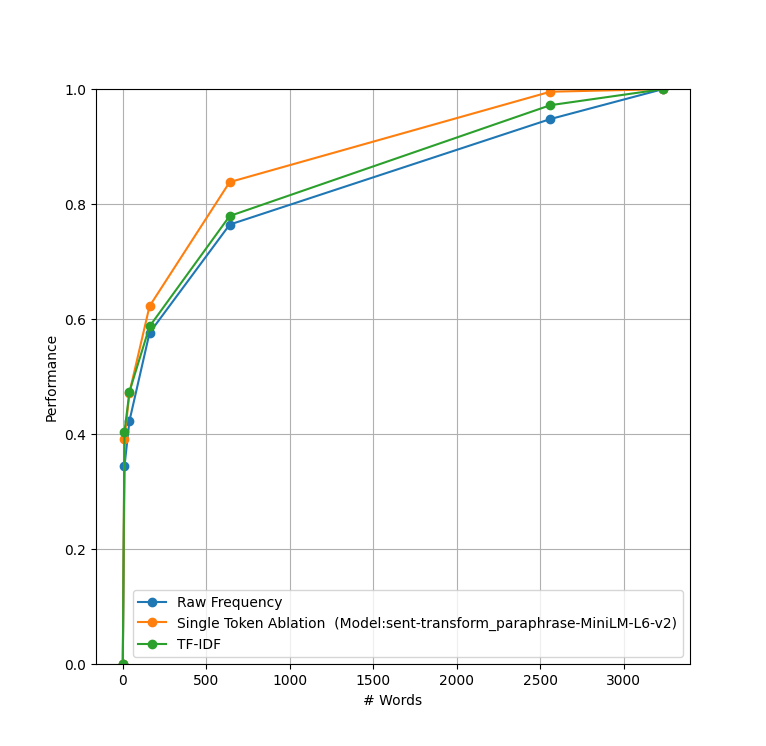
\includegraphics[width=0.5\textwidth]{marlon-brando-eval.png}
	\caption{Efficiency evaluation results on vocabulary lists for the Wikipedia Article of American actor Marlon Brando \protect\footnotemark.}
	\label{fig:marlon-brando-eval}
\end{figure}

\footnotetext{\url{https://en.wikipedia.org/wiki/Marlon_Brando}}

To make the figure readable, only three list generation approaches are compared, namely Raw Frequency, TF-IDF, and Single Token Ablation with the sentence embedding model.
We first evaluate the AI model performing the task with a vocabulary size of zero, simulating the state of not knowing any words.
The only tokens in this run are named entities and punctuation, as these are not considered to be potential vocabulary terms.
The vocabularies are then evaluated with an initial size of 10, and increase by a factor of 4 in each step, until a final evaluation is done with the full vocabulary list.
The full list typically contains all words from the corpus, which is why the performance reaches 1 with all lists.
To compare the results on a broader scale, we aggregate the results of the evaluation runs for each corpus type, word utility evaluation method and AI model (where applicable) by taking the average performance of the generated vocabulary list, with vocabulary sizes 0, 10, 40, 160, and 640.

\subsubsection{Utility Aggregation for Large Context Scenario}
\todo{the following is supposed to describe aggregation both for gen and eval. Make it understandable.}
As described above, the utility of a word for a given single corpus is calculated by taking the sum of the word's utility across the corpus' lines
For the large context evaluation scenario, we must also aggregate the utilities across corpora.
The simplest method would be to simply take the sum of each word's utility across all lines in the composite corpus.
However, this approach is biased against small single corpora, which contain fewer lines and are thus assigned less total word utility.
For this reason, we normalize the word utilities such that each corpus contributes the same total word utility.
For the evaluation too, we average over the performance scores of a list across corpora instead of across lines.

When we find two approaches for list generation produces vocabulary lists of similar efficiencies, we might ask ourselves if these lists are similar:
Can two lists which differ substantially in their ordering produce similar performance?
To answer this question, the next section introduces additional evaluation metrics which measure the similarity of two lists.


\subsection{List Similarity}
Apart from our own vocabulary list evaluation approach that measures performance of an AI model using the vocabulary list, we also compare how similar the lists are in general.
In order to compare the similarity of the resulting vocabulary lists provided by our approaches, metrics are needed that can be consistently calculated across the different approaches.
While a human may be able to qualitatively analyze lists and gain a rough idea of their similarity, computed metrics provide an instantaneous (if simplified) outlook on similarities.
A metric shall be defined as a function which takes as parameters two word lists of equal length which are word lists ordered in descending order by supposed utility, and outputs a real number giving either a distance or similarity between the lists.

Considerations of the choice of metric are:

\begin{description}
	\item [Handling of lists with partial overlap.]
	      Metrics must be able to handle elements which occur in only one of the two lists.
	      Thus, a metric which solely compares ranks of elements is not viable.
	\item [Start of lists is more impactful than end.]
	      Since the beginning of lists contains the words which are ranked as most important, changes at the top should impact the metric more than changes at the bottom. This includes (1) Equal differences in rank should be counted as more important if they occur further up the list.
	      A word that is rank 1 in list A, but rank 101 in list B says more about the similarity than if a word is rank 2000 in list A, but rank 2100 in list B. Likewise, if a word is absent from list B, it implies a greater difference if that word is at rank 1 in list A than if it were at rank 1000.
\end{description}

\subsubsection{Metrics Used}

\begin{description}
	\item [Sequential rank agreement (modified)] \cite{ekstromSequentialRankAgreement2015}: This metric is based on the deviations of some subset of the lists in the upper ranks.
	      It is important to note that this metric has an additional parameter "depth" which determines how many elements (from the top of the list) are considered.
	      It is therefore more helpful to view its results at various depths.
	      The original formula for this metric in the case of two lists is:
	      \[
		      a_{d} := a \text{ from start to rank } d
	      \]

	      \[
		      S_{d} := a_{d} \cup b_{d}
	      \]

	      \[
		      SRA_{d}(a, b) := \lambda \cdot \frac{\sum_{x \in S_{d}} \sigma ^2 \left( \left( r_{b}(x) \right) - \left( r_{a}(x) \right) \right)}{|S_{d}|}
	      \]

	      where \(\lambda\) is a normalization factor ensuring that \(\max(SRA) = 1\).
	      In its proposed form, this metric can only compare lists which contain the same set of unique elements, just in different orders.
	      In order to make it work on lists where this is not the case, one can set the "rank" of nonexisting elements to a value greater than the length of the lists, such as \(2 |a|\).
	      Another drawback of the metric is that the standard deviation of two numbers does not depend on their absolute value, only their difference.
	      However, to satisfy number 3 of the stated requirements, we can take the deviation of the logarithm of the ranks instead of the deviation of the ranks themselves, resulting in the formula

	      \[
		      r^{\prime}(x) :=
		      \begin{cases}
			      \mathrm{rank}_{b}(x) & \text{if } x \in b, \\
			      2 \cdot |a|          & \text{otherwise.}
		      \end{cases}
	      \]

	      \[
		      SRA^{mod}_{d}(a, b) := \lambda \cdot \frac{\sum_{x \in S_{d}} \sigma ^2 \left( \log (r^{\prime}_{b}(x))-\log(r^{\prime}_{a}(x))\right)}{|S_{d}|}
	      \]

	      For this modified version, \(\lambda\) can be calculated with:

	      \[
		      \lambda = \frac{1}{SRA_{d}(a, a^{*})},
	      \]

	      where \(a^{*}\) is a list such that \(a \cap a^{*} = \emptyset\).
	      % \item \textbf{Average overlap / rank-biased overlap} \cite{webberSimilarityMeasureIndefinite2010}: Compares ranked list and puts more emphasis on the top of the list than at the bottom. However, assumes that the elements of both lists are the same, i.e., that all elements of list A are also in list B and vice versa.
	      %
	      % \item \textbf{11-point interpolated average precision} \cite{manningIntroductionInformationRetrieval2008}: Uses set metric precision (though may also use recall or F1 score on various subsets of the list (first 10\%, first 20\% etc.) and takes their geometric mean to arrive at a single number.
	      %       As each of the elevent numbers is calculated on the partial subset of the list's elements starting at the first element, this means that changes in the top of the list affect more of these numbers and thus have a larger impact on the final calculated mean.
	      %       One drawback of this method is that precision measurement within the 10\% interval only takes into account set membership, not the order of words:
	      %       For a list containing 10,000 words, the evaluated intervals are words in the index intervals $\left[ 0, 1000 \right), \left[ 0, 2000 \right), ... ,\left[ 0, 10000 \right)$.  Differences of order within the first 1000 words are thus ignored.

	\item [Discounted Cumulative Gain]:
	      This formula outputs a value between 0 and 1, with 1 being given if both lists are identical, 0 when they have no elements in common, and values in between when there is partial overlap between elements and/or their order is different.
	      ${DCG_{p}} =\sum _{i=1}^{p}{\frac {rel_{i}}{\log _{2}(i+1)}}=rel_{1}+\sum _{i=2}^{p}{\frac {rel_{i}}{\log _{2}(i+1)}}$
\end{description}

\[
	rel_{i} :=
	\begin{cases}
		\frac{1}{rank_{b}(el_{i}) + 1} & \text{if } el_{i} \in b \\
		0                              & \text{otherwise}
	\end{cases}
\]
\subsubsection{Metrics Rejected}
\begin{description}
	\item [Kendall rank correlation ] \cite{kendallNEWMEASURERANK1938b}: This metric is bounded between 0 and 1 and compares the ranks of the elements of two lists. However, it cannot handle elements that only occur in one of the two lists, and thus is not suitable for our purposes. It also does not distinguish between differences in the upper and lower parts of the lists.
	\item [Spearman's footrule] \cite{spearmanCorrelationCalculatedFaulty1910}: Rejected for the same reasons as Kendall rank correlation.
\end{description}





\section{Baselines}
It may be useful to compare the lists generated by the various approaches with existing word lists from educational materials:
Textbooks often feature chapters with word lists, or sentences which can be converted to word lists with a tokenizer.
The purpose is to have a point of comparison, to see if generated lists agree with existing lists, and find reasons for differences.

\subsection{Existing Lists}
As one point of comparison, we can use existing vocabulary lists that are readily available in digital format, regardless of the method which created them.
For this, a survey was performed on popular language learning tools which make public some of their learning data.
However, mostly due to paywall restrictions, we only obtained one list for comparison, from the online learning platform \Rosetta (details below).

\subsection{Textbooks}
An obvious source of vocabulary lists to compare our lists against are English textbooks, which often contain vocabulary lists for each lesson.
However, the books we considered as candidates do not publish their course contents free of charge.
This includes:
\begin{itemize}
	\item \textit{Practical English Usage} by Michael Swan \footnote{Available at Oxford University Press at \url{https://elt.oup.com/catalogue/items/global/grammar_vocabulary/practical_english_usage_4th_edition/9780194202510} (last accessed on April 25, 2025)}
\end{itemize}

\subsubsection{Cambridge Word Lists}
Cambridge publishes word lists for certain levels of English \footnote{\url{https://www.cambridgeenglish.org/images/149681-yle-flyers-word-list.pdf}}.
However, these lists are meant for assessing learner's level of vocabulary skills, and the list for each level is ordered by alphabetical order, rather than the perceived level of the word, making them unusable as comparison to our approach.

\subsubsection{Duolingo}
While Duolingo is the most popular language learning application as of 2024, it does not publish its word lists or course contents that is free of cost and easily convertible to a format that can be processed with NLP tools.

\subsubsection{Rosetta Stone}
\Rosetta \footnote{\url{https://rosettastone.co.jp/}} is a popular online and mobile language learning platform.
\Rosetta\ publishes some of the course contents on its website \footnote{\url{https://support.rosettastone.com/s/article/Rosetta-Stone-Course-Contents}}.
These lessons take the form of phrases that should help a learner to quickly gain competence in their target language.
To make a list of vocabulary from \Rosetta 's lesson contents, we use the freely available lessons  of the \textit{American English} course (Units 1-20).
We convert the PDF files to text format, filter lines which do not contain lessons contents (e.g., "Lesson 8" and similar ancillary notes).
On the filtered text, we run the \texttt{bert-base-uncased} tokenizer and let the order of first appearance of a word in the lessons be its rank in the resulting vocabulary list.
Thus, the generated list features the lessons' words in the order in which \Rosetta\ introduces them to its learners, which presumably is close to the word order that \Rosetta estimates to be most useful.
One qualification of the previous statement is that some words may be introduced in order for the learner to have something concrete to talk about, rather than because of their estimated utility.
The final vocabulary list contains 2,545 words in total.

This section has introduced some pre-existing lists as points of comparison for our generated vocabulary lists.
However, one shortcoming of this comparison is that these lists have not been prepared with the same linguistic contexts in mind as those made by this work's approach, and thus their utility is naturally greater in general-context corpora than specialized ones.
While the context specificity of this work's utility extraction method is a major advance for creating vocabulary lists, it also makes this an unfair comparison.

However, apart from pre-existing lists, there also exist pre-existing \textbf{methods} of finding important words in texts, which we can also use as baselines to compare with our method.
These also use corpora, but not AI models or XAI methods to find important words.
The next section introduces some of these methods, which we use to generate comparison lists to our own.


\subsection{Frequency-Based List Generation Methods}
To get an impression of how well our XAI-based method for vocabulary list generation performs, we employ the three frequency-based methods for generating lists of vocabulary introduced in Section \ref{sec:frequency-based-list-generation-methods}, namely Raw Frequency, Average Reduced Frequency, and TF-IDF.
We use these three measures as baselines to our methods, using the same tokenizer \texttt{bert-base-uncased} to divide texts into words that we can count.
To calculate the inverse document frequency in TF-IDF, we use a random sample of 53,178 documents from the Oscar corpus (see Section \ref{sec:oscar}).


\subsection{LLM Prompt}
In recent years, Large Language Models have become a popular tools for language learners to find new words to learn about specific areas.
For this purpose, we run the following prompt to ChatGPT 3 for each context to get a sense of how well our method performs against this easy method.

Prompt:

\begin{lstlisting}[caption={Prompt given to the language model.}, label={lst:blade_runner_prompt}, captionpos=b]
	Given a learner of English who knows no English words so far:
Give me a list of 50 words from the script of the movie "Blade Runner" that they can learn, such that when reading the full script, they have the best understanding of what they are reading.
Order the list such that the most useful words appear at the top.
Do not group the words, just generate a raw list.
Do not number the bullet points. Do not put hyperlinks in the list.

\end{lstlisting}
\todo{results}

\section{Results} \label{sec:results}

\subsection{Correspondence of Efficiency Evaluation with Human Intuition}
As mentioned in the introduction to this chapter, we use the performance of AI models on corpora where we simulate a limited vocabulary in order to measure the efficiency of a vocabulary list.
Before we present the results of these tests, however, we examine whether the performance of AI models is a reliable indicator that the list is useful to humans as well.
This section therefore examines several vocabulary lists tested on a short sample text containing ten lines of dialog from the subtitles of the 1972 movie \textit{The Godfather}, seen here:

\begin{lstlisting}[caption={
Sample text.
}, label={lst:sample-text-original}
, captionpos=b]
Moe loves the business.
He never said nothing about selling.
I'll make him an offer he can't refuse.
See, Johnny...
We figure that entertainment would draw gamblers to the casino.
We hope you'll sign a contract to appear five times a year.
Perhaps convince some of your friends in the movies to do the same.
We're counting on you.
Sure, Mike.
I'll do anything for my godfather.
\end{lstlisting}




After preprocessing the text and leaving only the named entities and punctuation tokens in the text (which constitutes our starting point for the evaluation), the text becomes as follows (evaluation score for each line are displayed on the left):


\begin{lstlisting}[caption={
Sample text with no vocabulary. Total score: 0.17.
}, label={lst:sample-text-empty}
, captionpos=b]
0.0	                      .
0.0	                                   .
0.0	 '                            '         .
0.9	   ,johnny...
0.0	                                                              .
0.0	           '                                               .
0.0	                                                                  .
0.0	  '                   .
0.8	    ,mike.
0.0	 '                                .
\end{lstlisting}




Due to the uncased tokenizer used, all words in the reconstructed text are lowercase.
We can see that the lines containing named entities (Line 4 and 9) already have a rather high score in the evaluation, reflecting the importance of the names to the meaning of the sentences.
However, the other lines receive a score of 0.0, resulting in an overall score of 0.17.
We also observe that the name \textit{Moe} in line 1 is not recognized by the \texttt{spacy} named entity recognizer (falsely) making it a possible vocabulary word.

To compare their intuitive utilities, we use four vocabulary lists on the corpus and see how well their first words perform when evaluated on the sample text:
\begin{enumerate}
	\item A randomly ordered list from words in the sample text.
	\item A list compiled with raw frequency.
	\item A list compiled with TF-IDF (with the Oscar corpus as normalization).
	\item A list compiled by Single Token Summary with sentence embedding.
\end{enumerate}

The tops of the lists can be seen in Table \ref{tbl:first-k-words-sample}.

\begin{table}[H]
	\centering
	\begin{tabular}{lllll}
\toprule
 & \rotatebox{90}{Random} & \rotatebox{90}{Raw Frequency} & \rotatebox{90}{TF-IDF} & \rotatebox{90}{Single Token Summary - Sent. Emb.} \\
\midrule
0 & i & the & moe & moe \\
1 & a & ll & godfather & casino \\
2 & selling & we & gamblers & godfather \\
3 & same & to & ll & gamblers \\
4 & contract & he & convince & counting \\
5 & make & i & counting & offer \\
6 & draw & you & casino & refuse \\
7 & of & a & refuse & ll \\
8 & appear & do & loves & contract \\
9 & casino & moe & draw & movies \\
\bottomrule
\end{tabular}
	\caption{Top 10 words of each compared list on the sample text.}
	\label{tbl:first-k-words-sample}
\end{table}

It can be seen that the ten top words of the lists collected with TF-IDF and the XAI Single Token Summary give a better idea of the meaning of the text than the words from the random and frequency lists.
Next, we examine the words in the context of the sample text.
In the following listings, we see the sample text with the 10 top words filled in from each vocabulary list, in addition to the recognized named entities.
Each line displays the evaluation score for it, and the total score (calculated by taking the average across the lines) is seen in the caption of each listing.


\begin{lstlisting}[caption={
Sample text with 10 words from the Random list. Total score: 0.3.
}, label={lst:sample-text-random}
, captionpos=b]
0.0	                      .
0.2	                            selling.
0.0	i'    make                    '         .
0.9	   ,johnny...
0.7	                                   draw                 casino.
0.3	           '         a contract    appear            a     .
0.1	                      of                                      same.
0.0	  '                   .
0.8	    ,mike.
0.1	i'                                .
\end{lstlisting}




\begin{lstlisting}[caption={
Sample text with 10 words from the Raw Frequency list. Total score: 0.33.
}, label={lst:sample-text-frequency}
, captionpos=b]
0.6	moe       the         .
0.1	he                                 .
0.3	i' ll                   he    '         .
0.9	   ,johnny...
0.1	we                                               to the       .
0.1	we      you' ll      a          to                   a     .
0.1	                                         the        to do the     .
0.3	we'                you.
0.8	    ,mike.
0.2	i' ll do                          .
\end{lstlisting}




\begin{lstlisting}[caption={
Sample text with 10 words from the TF-IDF list. Total score: 0.52.
}, label={lst:sample-text-tf-idf}
, captionpos=b]
0.8	moe loves             .
0.0	                                   .
0.5	 ' ll                         '   refuse.
0.9	   ,johnny...
0.7	                                   draw gamblers        casino.
0.1	           ' ll                                            .
0.3	        convince                                                  .
0.5	  '    counting       .
0.8	    ,mike.
0.6	 ' ll                    godfather.
\end{lstlisting}




\begin{lstlisting}[caption={
Sample text with 10 words from the Single Token Summary list. Total score: 0.56.
}, label={lst:sample-text-single-token-summary}
, captionpos=b]
0.7	moe                   .
0.0	                                   .
0.7	 ' ll             offer       '   refuse.
0.9	   ,johnny...
0.7	                                        gamblers        casino.
0.4	           ' ll        contract                            .
0.4	                                             movies               .
0.5	  '    counting       .
0.8	    ,mike.
0.6	 ' ll                    godfather.
\end{lstlisting}




The main observation is that the texts with the TF-IDF and Single Token Summary resemble the meaning of the original text much closer than the other two approaches, and are indeed evaluated significantly higher (0.52 and 0.56 vs. 0.33 and 0.30).
In our opinion, this is evidence that our evaluation scores roughly coincide with how much the words let a reader understand the text, aligning with utility as defined in Section \ref{sec:utility}.
Both of these lists feature the essential words \textit{casino}, \textit{godfather} and \textit{gamblers}, as well as other words which let a reader guess at the situation.

We can, however, also notice some peculiarities in the evaluation scores:
The text with words from the randomly assembled list (Listing \ref{lst:sample-text-random}) seems more understandable to us than when words from the  frequency list are filled in (Listing \ref{lst:sample-text-frequency}), since the randomly compiled list contains useful words such as \textit{selling}, \textit{casino} and \textit{contract}.
However, the text with the frequency words receives a higher evaluation score than the one with the random words (0.33 vs. 0.3).
This is due partially to the unrecognized entity \textit{moe} which is contained in the frequency list but not the random one, "artificially" boosting the score of the frequency list.
But even disregarding that name, the scores are not as disparate as we expected them to be:
For example, line 3 in the random words text \textit{"i' make       ."} receives a (rounded) score of 0.0, while the same line in the frequency text \textit{"i' ll      he      ."} is assigned a score of 0.3.
Since both versions of the line seem to contain very little information, this difference in the evaluation score suggests that the evaluation scores do not reflect the true utility of words in all circumstances.
With these observations in mind, we present the evaluation results in the next sections.

\subsection{Small Context} \label{sec:results-small-context}
This section shows the results of our evaluation approach for the efficiencies of vocabulary list, applied to lists which have been generated by the various list generation approaches.
Performance scores were rounded to two decimals to improve readability.


Table \ref{tbl:performance-results-single-opensubs} and \ref{tbl:performance-results-single-wikipedia} show the aggregated results of small-scale corpora, separated by corpus type.
For small corpora, there is no train-test-data distinction, thus for each corpus and extraction method, a vocabulary list produced, whose efficiency is then evaluated with the same corpus as a basis.
%
% \begin{table}[ht]
% 	\centering
% 	\begin{tabular}{llrrrrrrrr}
\toprule
 &  & \multicolumn{4}{r}{Performance} & \multicolumn{4}{r}{Performance ($\sigma$)} \\
 & Vocabulary Size & 10 & 40 & 160 & 640 & 10 & 40 & 160 & 640 \\
Generation Method & Generation Model &  &  &  &  &  &  &  &  \\
\midrule
Raw Frequency & - & 0.14 & 0.30 & 0.60 & 0.88 & 0.14 & 0.25 & 0.31 & 0.21 \\
\cline{1-10}
Average Reduced Frequency & - & 0.14 & 0.29 & 0.58 & 0.88 & 0.14 & 0.24 & 0.31 & 0.21 \\
\cline{1-10}
TF-IDF & - & 0.18 & 0.33 & 0.60 & 0.89 & 0.23 & 0.30 & 0.31 & 0.19 \\
\cline{1-10}
Attention & sent-transform\_paraphrase-MiniLM-L6-v2 & 0.17 & 0.33 & 0.62 & 0.92 & 0.20 & 0.29 & 0.31 & 0.16 \\
\cline{1-10}
Single Token Ablation & sent-transform\_paraphrase-MiniLM-L6-v2 & 0.19 & 0.35 & 0.64 & 0.94 & 0.23 & 0.30 & 0.31 & 0.12 \\
\cline{1-10}
Single Token Summary & sent-transform\_paraphrase-MiniLM-L6-v2 & 0.14 & 0.27 & 0.56 & 0.84 & 0.14 & 0.23 & 0.31 & 0.25 \\
\cline{1-10}
Progressive Summary & sent-transform\_paraphrase-MiniLM-L6-v2 & 0.18 & 0.31 & 0.63 & 0.93 & 0.24 & 0.30 & 0.31 & 0.12 \\
\cline{1-10}
\midrule
\textbf{Mean} & \textbf{-} & \textbf{0.16} & \textbf{0.31} & \textbf{0.60} & \textbf{0.90} & \textbf{0.19} & \textbf{0.27} & \textbf{0.31} & \textbf{0.1} \\
\cline{1-10}
\bottomrule
\end{tabular}


% \begin{tabular}{llrrrrrrrr}
% \toprule
%  &  & \multicolumn{4}{r}{performance} & \multicolumn{4}{r}{performance\_std} \\
%  & vocab\_size & 10 & 40 & 160 & 640 & 10 & 40 & 160 & 640 \\
% generation\_method & generation\_model &  &  &  &  &  &  &  &  \\
% \midrule
% frequency & - & 0.14 & 0.29 & 0.59 & 0.88 & 0.15 & 0.25 & 0.31 & 0.21 \\
% \cline{1-10}
% average-reduced-frequency & - & 0.14 & 0.28 & 0.58 & 0.88 & 0.14 & 0.24 & 0.31 & 0.21 \\
% \cline{1-10}
% tf-idf & - & 0.18 & 0.32 & 0.59 & 0.89 & 0.23 & 0.30 & 0.32 & 0.19 \\
% \cline{1-10}
% attention & sent-transform\_paraphrase-MiniLM-L6-v2 & 0.17 & 0.33 & 0.62 & 0.92 & 0.20 & 0.29 & 0.31 & 0.16 \\
% \cline{1-10}
% single-token-ablation & sent-transform\_paraphrase-MiniLM-L6-v2 & 0.19 & 0.35 & 0.64 & 0.94 & 0.23 & 0.30 & 0.31 & 0.12 \\
% \cline{1-10}
% single-token-summary & sent-transform\_paraphrase-MiniLM-L6-v2 & 0.14 & 0.27 & 0.56 & 0.84 & 0.14 & 0.23 & 0.31 & 0.25 \\
% \cline{1-10}
% summaries & sent-transform\_paraphrase-MiniLM-L6-v2 & 0.17 & 0.29 & 0.61 & 0.93 & 0.24 & 0.30 & 0.32 & 0.12 \\
% \cline{1-10}
% \bottomrule
% \end{tabular}

% 	\caption{DELETE THIS}
% \end{table}


\begin{table}[H]
	\centering
	\resizebox{\textwidth}{!}{%
		\begin{tabular}{lrrrrr}
\toprule
 & Size=0 & Size=10 & Size=40 & Size=160 & Size=640 \\
\midrule
Raw Frequency & \cellcolor[RGB]{58,76,192}0.16 & \cellcolor[RGB]{85,113,222}0.23 & \cellcolor[RGB]{141,175,253}0.36 & \cellcolor[RGB]{241,203,184}0.63 & \cellcolor[RGB]{202,61,56}0.90 \\
Average Reduced Frequency & \cellcolor[RGB]{58,76,192}0.16 & \cellcolor[RGB]{85,113,222}0.23 & \cellcolor[RGB]{141,175,253}0.36 & \cellcolor[RGB]{239,206,188}0.62 & \cellcolor[RGB]{202,61,56}0.90 \\
TF-IDF & \cellcolor[RGB]{58,76,192}0.16 & \cellcolor[RGB]{88,118,226}0.24 & \cellcolor[RGB]{151,184,254}0.38 & \cellcolor[RGB]{241,203,184}0.63 & \cellcolor[RGB]{197,50,51}0.91 \\
Attention - Sent. Emb. & \cellcolor[RGB]{58,76,192}0.16 & \cellcolor[RGB]{88,118,226}0.24 & \cellcolor[RGB]{151,184,254}0.38 & \cellcolor[RGB]{242,200,179}0.64 & \cellcolor[RGB]{202,61,56}0.90 \\
Single Token Ablation - Sent. Emb. & \cellcolor[RGB]{58,76,192}0.16 & \cellcolor[RGB]{97,130,234}0.26 & \cellcolor[RGB]{159,190,254}0.40 & \cellcolor[RGB]{246,189,164}0.67 & \cellcolor[RGB]{179,3,38}0.95 \\
Single Token Summary - Sent. Emb. & \cellcolor[RGB]{58,76,192}0.16 & \cellcolor[RGB]{97,130,234}0.26 & \cellcolor[RGB]{164,194,254}0.41 & \cellcolor[RGB]{245,193,168}0.66 & \cellcolor[RGB]{184,17,41}0.94 \\
Progressive Summary - Sent. Emb. & \cellcolor[RGB]{58,76,192}0.16 & \cellcolor[RGB]{93,125,230}0.25 & \cellcolor[RGB]{159,190,254}0.40 & \cellcolor[RGB]{245,193,168}0.66 & \cellcolor[RGB]{184,17,41}0.94 \\
\midrule
{[Mean]} & \cellcolor[RGB]{58,76,192}0.16 & \cellcolor[RGB]{91,121,228}0.24 & \cellcolor[RGB]{152,185,254}0.38 & \cellcolor[RGB]{242,199,178}0.64 & \cellcolor[RGB]{193,42,48}0.92 \\
\bottomrule
\end{tabular}
	}
	\caption{Model performance across vocabulary sizes on single subtitles.}
	\label{tbl:performance-results-single-opensubs}
\end{table}

\begin{table}[H]
	\centering
	\resizebox{\textwidth}{!}{%
		\begin{tabular}{lrrrrr}
\toprule
 & Size=0 & Size=10 & Size=40 & Size=160 & Size=640 \\
\midrule
Raw Frequency & \cellcolor[RGB]{58,76,192}\textbf{0.53} & \cellcolor[RGB]{101,134,236}0.58 & \cellcolor[RGB]{171,199,252}0.67 & \cellcolor[RGB]{242,199,178}0.79 & \cellcolor[RGB]{218,90,72}0.91 \\
Average Reduced Frequency & \cellcolor[RGB]{58,76,192}\textbf{0.53} & \cellcolor[RGB]{100,133,235}0.58 & \cellcolor[RGB]{167,196,253}0.67 & \cellcolor[RGB]{240,204,185}0.78 & \cellcolor[RGB]{220,94,75}0.91 \\
TF-IDF & \cellcolor[RGB]{58,76,192}\textbf{0.53} & \cellcolor[RGB]{135,170,252}0.63 & \cellcolor[RGB]{194,212,243}0.70 & \cellcolor[RGB]{246,189,164}0.81 & \cellcolor[RGB]{210,75,63}0.92 \\
Attention - Sent. Emb. & \cellcolor[RGB]{58,76,192}\textbf{0.53} & \cellcolor[RGB]{109,144,241}0.60 & \cellcolor[RGB]{182,206,249}0.69 & \cellcolor[RGB]{246,185,157}0.81 & \cellcolor[RGB]{201,59,55}0.93 \\
Single Token Ablation - NSP & \cellcolor[RGB]{58,76,192}\textbf{0.53} & \cellcolor[RGB]{103,136,237}0.59 & \cellcolor[RGB]{170,198,253}0.67 & \cellcolor[RGB]{241,202,182}0.79 & \cellcolor[RGB]{223,100,79}0.90 \\
Single Token Ablation - Sent. Emb. & \cellcolor[RGB]{58,76,192}\textbf{0.53} & \cellcolor[RGB]{139,174,253}0.63 & \cellcolor[RGB]{208,218,233}0.72 & \cellcolor[RGB]{244,154,123}\textbf{0.85} & \cellcolor[RGB]{179,3,38}\textbf{0.96} \\
Single Token Summary - Sent. Emb. & \cellcolor[RGB]{58,76,192}\textbf{0.53} & \cellcolor[RGB]{148,181,254}\textbf{0.64} & \cellcolor[RGB]{211,219,230}\textbf{0.73} & \cellcolor[RGB]{246,163,132}0.84 & \cellcolor[RGB]{196,48,50}0.94 \\
Progressive Summary - Sent. Emb. & \cellcolor[RGB]{58,76,192}\textbf{0.53} & \cellcolor[RGB]{134,169,252}0.63 & \cellcolor[RGB]{201,215,238}0.71 & \cellcolor[RGB]{246,167,137}0.83 & \cellcolor[RGB]{190,35,45}0.95 \\
\midrule 
\textbf{[Mean]} & \textbf{0.53} & \textbf{0.61} & \textbf{0.69} & \textbf{0.81} & \textbf{0.93} \\
\bottomrule
\end{tabular}
	}
	\caption{Model performance across vocabulary sizes on single Wikipedia articles.}
	\label{tbl:performance-results-single-wikipedia}
\end{table}

\begin{table}[H]
	\centering
	\resizebox{\textwidth}{!}{%
		\begin{tabular}{lrrrrrrrrr}
\toprule
 & \rotatebox{90}{Raw Frequency} & \rotatebox{90}{Average Reduced Frequency} & \rotatebox{90}{TF-IDF} & \rotatebox{90}{Attention - Sent. Emb.} & \rotatebox{90}{Single Token Ablation - NSP} & \rotatebox{90}{Single Token Ablation - Sent. Emb.} & \rotatebox{90}{Single Token Summary - Sent. Emb.} & \rotatebox{90}{Progressive Summary - Sent. Emb.} & \rotatebox{90}{Random} \\
\midrule
Raw Frequency & \cellcolor[RGB]{0,0,0}nan & \cellcolor[RGB]{179,3,38}0.99 & \cellcolor[RGB]{182,206,249}0.64 & \cellcolor[RGB]{214,82,67}0.94 & \cellcolor[RGB]{184,17,41}0.98 & \cellcolor[RGB]{234,211,199}0.74 & \cellcolor[RGB]{206,217,235}0.68 & \cellcolor[RGB]{190,211,245}0.65 & \cellcolor[RGB]{108,142,241}0.52 \\
Average Reduced Frequency & \cellcolor[RGB]{179,3,38}0.99 & \cellcolor[RGB]{0,0,0}nan & \cellcolor[RGB]{176,203,251}0.63 & \cellcolor[RGB]{215,84,68}0.93 & \cellcolor[RGB]{185,22,42}0.98 & \cellcolor[RGB]{231,214,204}0.74 & \cellcolor[RGB]{202,216,238}0.68 & \cellcolor[RGB]{187,209,247}0.65 & \cellcolor[RGB]{105,139,239}0.52 \\
TF-IDF & \cellcolor[RGB]{182,206,249}0.64 & \cellcolor[RGB]{176,203,251}0.63 & \cellcolor[RGB]{0,0,0}nan & \cellcolor[RGB]{168,197,253}0.62 & \cellcolor[RGB]{117,152,246}0.54 & \cellcolor[RGB]{246,183,156}0.80 & \cellcolor[RGB]{246,166,135}0.83 & \cellcolor[RGB]{244,195,171}0.78 & \cellcolor[RGB]{63,83,198}0.44 \\
Attention - Sent. Emb. & \cellcolor[RGB]{214,82,67}0.94 & \cellcolor[RGB]{215,84,68}0.93 & \cellcolor[RGB]{168,197,253}0.62 & \cellcolor[RGB]{0,0,0}nan & \cellcolor[RGB]{205,66,58}0.95 & \cellcolor[RGB]{242,199,178}0.77 & \cellcolor[RGB]{220,220,221}0.71 & \cellcolor[RGB]{194,212,243}0.66 & \cellcolor[RGB]{0,0,0}nan \\
Single Token Ablation - NSP & \cellcolor[RGB]{184,17,41}0.98 & \cellcolor[RGB]{185,22,42}0.98 & \cellcolor[RGB]{117,152,246}0.54 & \cellcolor[RGB]{205,66,58}0.95 & \cellcolor[RGB]{0,0,0}nan & \cellcolor[RGB]{149,183,254}0.58 & \cellcolor[RGB]{135,170,252}0.56 & \cellcolor[RGB]{67,90,204}0.45 & \cellcolor[RGB]{0,0,0}nan \\
Single Token Ablation - Sent. Emb. & \cellcolor[RGB]{234,211,199}0.74 & \cellcolor[RGB]{231,214,204}0.74 & \cellcolor[RGB]{246,183,156}0.80 & \cellcolor[RGB]{242,199,178}0.77 & \cellcolor[RGB]{149,183,254}0.58 & \cellcolor[RGB]{0,0,0}nan & \cellcolor[RGB]{230,114,89}0.90 & \cellcolor[RGB]{243,152,121}0.85 & \cellcolor[RGB]{58,76,192}0.43 \\
Single Token Summary - Sent. Emb. & \cellcolor[RGB]{206,217,235}0.68 & \cellcolor[RGB]{202,216,238}0.68 & \cellcolor[RGB]{246,166,135}0.83 & \cellcolor[RGB]{220,220,221}0.71 & \cellcolor[RGB]{135,170,252}0.56 & \cellcolor[RGB]{230,114,89}0.90 & \cellcolor[RGB]{0,0,0}nan & \cellcolor[RGB]{246,166,135}0.83 & \cellcolor[RGB]{69,91,205}0.45 \\
Progressive Summary - Sent. Emb. & \cellcolor[RGB]{190,211,245}0.65 & \cellcolor[RGB]{187,209,247}0.65 & \cellcolor[RGB]{244,195,171}0.78 & \cellcolor[RGB]{194,212,243}0.66 & \cellcolor[RGB]{67,90,204}0.45 & \cellcolor[RGB]{243,152,121}0.85 & \cellcolor[RGB]{246,166,135}0.83 & \cellcolor[RGB]{0,0,0}nan & \cellcolor[RGB]{69,91,205}0.45 \\
Random & \cellcolor[RGB]{108,142,241}0.52 & \cellcolor[RGB]{105,139,239}0.52 & \cellcolor[RGB]{63,83,198}0.44 & \cellcolor[RGB]{0,0,0}nan & \cellcolor[RGB]{0,0,0}nan & \cellcolor[RGB]{58,76,192}0.43 & \cellcolor[RGB]{69,91,205}0.45 & \cellcolor[RGB]{69,91,205}0.45 & \cellcolor[RGB]{0,0,0}nan \\
\bottomrule
\end{tabular}
	}
	\caption{Similarity of vocabulary lists. Black boxes represent missing values.}
	\label{tbl:similarity-results-single}
\end{table}



We can observe several points in the data:

Single Token Ablation with sentence embedding achieves the highest results across corpus types.
It is also among the approaches with the least spread of performance, as seen by the standard deviation of the corpora scores.
Since the model used for list generation and list evaluation is the same,
What we can gleam from this fact is that the utilities calculated from individual lines, when aggregated over the dataset, approach the word utilities with respect to the entire corpus better than frequency-based approaches.

The Progressive Summary approach, despite being a more complex approach, does not outperform Single Token Ablation.
The comparison is difficult, as the calculation of line utilities for Progressive Summary is not as straightforward as for Single Token Ablation.
However, Progressive Summary has the additional disadvantage of requiring a much greater amount of time to calculate for a corpus.
For this reason, it seems that investigating possible improvements for how line utilities can be aggregated to calculate corpus utility may not be productive.

Single Token Summary produced the lowest performance across corpus types and vocabulary sizes, falling short of even the frequency-based baselines.
This may be due to the fact that it does not take into account relationships between words in the sentence, as each summary contains only a single word.
For this reason, Single Token Summary seems to be of very limited potential for word utility evaluation.

TF-IDF, despite its simplicity, produces lists of an efficiency very close to the XAI methods, especially at low vocabulary sizes.
TF-IDF, while usually used to capture words characteristics of documents, also seems to capture useful words rather well.
This could be seen as evidence to the effect that, while learning words by their general frequency provides the best coverage of texts, the coverage is not a good proxy for measuring the understanding of a text.


For the transformer attention approach, both the model for next sentence prediction and the model for sentence embedding produce very similar results.
Because both models function with a BERT model at their core, this result is within the realm of expectation.
The slightly better performance of the NSP model may be due to its greater size (12 attention heads vs. 6 heads), but the difference is too slight to make a definitive judgement.

We can also observe that the type of corpus used had a significant impact on the model performance for small vocabulary sizes:
The average performance of 10- and 40-word-vocabularies was $0.37$ and $0.53$ for Wikipedia articles, but only $0.16$ and $0.30$ for subtitles, respectively.
The discrepancy in performance of small vocabulary sizes between the two corpus types may be due to the fact that Wikipedia articles address a particular \textit{topic}, meaning that knowing the main words (such as those from the article title) may produce a high initial boost in performance.
One piece of counter-evidence to this theory is that raw frequency also performs better on Wikipedia than on OpenSubtitles, despite frequency lists from both corpus types featuring many stopwords at their top.
An alternative hypothesis is that Wikipedia articles are more similar to the data the models had been trained on.
This cannot be confirmed, however, as the source of BERT's training data is not publicly known.
An interesting point to note is that, for a vocabulary size of 640, the list efficiencies nearly converge:
Despite the larger average corpus size of movie subtitles, the average performance is 0.90 for subtitles and 0.89 for Wikipedia.

\subsection{Large Context} \label{sec:results-large-context}
So far, we have analyzed the efficiencies of vocabulary lists with respect to the same corpus which was used to generate them in the first place.
This may be useful for a learner who wishes to read specific articles of watch specific movies, and learn the most useful vocabulary beforehand.
However, in real life, it is not always possible for a learner to know the exact contents of the texts they will be engaging in:
Natural conversations, for examples, are not deterministically predictable, and learners will likely wish to acquire abilities beyond the narrow scope of a few selected Wikipedia articles.
For this reason, we also test the efficiencies of vocabulary lists on corpora which are similar, but not the same as the source of their generation.

To model these linguistic contexts, we use Wikipedia categories:
For each category, we randomly split its articles into "train" and "test" articles, with a test percentage of 20\%.
When generating vocabulary lists, only the "train" articles are used as inputs.
With these lists, we evaluate the list efficiencies against the "test" corpora.
The scores across the individual corpora is then aggregated by taking the mean.
% Table \ref{tbl:performance-results-wikipedia-categories} shows the results of these experiments.

To first gain an overview of the resulting lists, we present the first 20 words of each vocabulary list made from the sample of 632 subtitles:

\begin{table}[H]
	\centering
	% \resizebox{\textwidth}{!}{%
	\begin{tabular}{llllllll}
\toprule
 & \rotatebox{90}{Raw Frequency} & \rotatebox{90}{Average Reduced Frequency} & \rotatebox{90}{TF-IDF} & \rotatebox{90}{Attention - Sent. Emb.} & \rotatebox{90}{Single Token Ablation - Sent. Emb.} & \rotatebox{90}{Single Token Summary - Sent. Emb.} & \rotatebox{90}{Progressive Summary - Sent. Emb.} \\
\midrule
0 & you & you & i & you & you & you & you \\
1 & i & i & you & i & i & i & i \\
2 & the & the & me & the & what & we & it \\
3 & to & to & t & s & it & it & what \\
4 & s & s & yeah & it & no & no & no \\
5 & a & a & okay & to & that & that & that \\
6 & it & it & m & no & know & what & we \\
7 & that & that & what & what & he & to & he \\
8 & and & t & he & that & we & t & s \\
9 & t & and & oh & a & me & here & me \\
10 & of & of & s & is & to & he & to \\
11 & we & is & re & and & this & go & the \\
12 & is & what & gonna & we & s & know & know \\
13 & what & in & don & yeah & the & yeah & is \\
14 & in & we & my & t & is & don & not \\
15 & me & me & it & this & right & okay & go \\
16 & this & this & know & me & come & not & here \\
17 & he & for & hey & okay & not & she & this \\
18 & your & on & we & of & do & her & t \\
19 & for & your & no & on & go & oh & okay \\
\bottomrule
\end{tabular}
	% }
	\caption{Top 20 words of the generated lists for the OpenSubtitles dataset.}
	\label{tbl:first-k-words-opensubs}
\end{table}

We can see some similarities across all lists:
Every list is headed by the two pronouns \textit{i} and \textit{you}, which seems reasonable for movie dialog.
After these, we can see the characteristics of the various approaches:
Raw Frequency and Average Reduced Frequency produce very similar lists, consisting mostly of stop words at the top.
The list made from using attention as explanation follows a similar pattern.
In contrast, the lists generated from both TF-IDF and feature importance explanations show words that are more useful for a beginner language learner in our view:
All of them contain at least one verb (\textit{know}), as well as several words that can constitute a meaningful sentence by themselves, such as \textit{what}, \textit{okay}, \textit{right}, \textit{yeah}.
Next, we present the results of the efficiency evaluation of the large lists produced on the (separate) test datasets.
We include the vocabulary list produced from the \Rosetta lesson in this evaluation, since both it and our own lists were not specifically compiled for the evaluation data (though our lists were compiled on more similar data).


\begin{table}[H]
	\centering
	\resizebox{\textwidth}{!}{%
		\begin{tabular}{lrrrrrr}
\toprule
 & Size=0 & Size=10 & Size=40 & Size=160 & Size=640 & Size=2560 \\
\midrule
Raw Frequency & \cellcolor[RGB]{58,76,192}0.16 & \cellcolor[RGB]{82,110,220}0.22 & \cellcolor[RGB]{134,169,252}0.33 & \cellcolor[RGB]{229,216,208}0.54 & \cellcolor[RGB]{236,128,100}0.74 & \cellcolor[RGB]{179,3,38}0.87 \\
Average Reduced Frequency & \cellcolor[RGB]{58,76,192}0.16 & \cellcolor[RGB]{82,110,220}0.22 & \cellcolor[RGB]{134,169,252}0.33 & \cellcolor[RGB]{229,216,208}0.54 & \cellcolor[RGB]{236,130,102}0.73 & \cellcolor[RGB]{179,3,38}0.87 \\
TF-IDF & \cellcolor[RGB]{58,76,192}0.16 & \cellcolor[RGB]{82,110,220}0.22 & \cellcolor[RGB]{137,172,252}0.33 & \cellcolor[RGB]{229,216,208}0.54 & \cellcolor[RGB]{235,127,99}0.74 & \cellcolor[RGB]{179,3,38}0.87 \\
Attention - Sent. Emb. & \cellcolor[RGB]{58,76,192}0.16 & \cellcolor[RGB]{86,115,224}0.23 & \cellcolor[RGB]{141,175,253}0.34 & \cellcolor[RGB]{231,214,205}0.55 & \cellcolor[RGB]{236,128,100}0.74 & \cellcolor[RGB]{181,8,39}0.87 \\
Single Token Ablation - Sent. Emb. & \cellcolor[RGB]{58,76,192}0.16 & \cellcolor[RGB]{87,117,225}0.23 & \cellcolor[RGB]{141,175,253}0.34 & \cellcolor[RGB]{233,212,201}\textbf{0.55} & \cellcolor[RGB]{234,125,97}\textbf{0.74} & \cellcolor[RGB]{179,3,38}\textbf{0.87} \\
Single Token Summary - Sent. Emb. & \cellcolor[RGB]{58,76,192}0.16 & \cellcolor[RGB]{90,120,227}\textbf{0.23} & \cellcolor[RGB]{145,179,254}\textbf{0.35} & \cellcolor[RGB]{232,213,202}0.55 & \cellcolor[RGB]{234,125,97}\textbf{0.74} & \cellcolor[RGB]{179,3,38}\textbf{0.87} \\
Progressive Summary - Sent. Emb. & \cellcolor[RGB]{58,76,192}0.16 & \cellcolor[RGB]{87,117,225}0.23 & \cellcolor[RGB]{144,178,254}0.35 & \cellcolor[RGB]{232,213,202}0.55 & \cellcolor[RGB]{235,127,99}0.74 & \cellcolor[RGB]{181,8,39}0.87 \\
rosetta & \cellcolor[RGB]{59,77,193}\textbf{0.17} & \cellcolor[RGB]{65,86,201}0.18 & \cellcolor[RGB]{73,98,211}0.20 & \cellcolor[RGB]{123,158,248}0.30 & \cellcolor[RGB]{197,213,242}0.46 & \cellcolor[RGB]{0,0,0}nan \\
\midrule 
\textbf{[Mean]} & \textbf{0.16} & \textbf{0.22} & \textbf{0.32} & \textbf{0.52} & \textbf{0.70} & \textbf{0.87} \\
\bottomrule
\end{tabular}
	}
	\caption{Model performance across vocabulary sizes on subtitles, with separate train/test subtitles.}
	\label{tbl:performance-results-opensubs-large}
\end{table}


\begin{table}[H]
	\centering
	\resizebox{\textwidth}{!}{%
		\begin{tabular}{lrrrrrr}
\toprule
 & Size=0 & Size=10 & Size=40 & Size=160 & Size=640 & Size=2560 \\
\midrule
Raw Frequency & \cellcolor[RGB]{58,76,192}0.53 & \cellcolor[RGB]{101,134,236}0.58 & \cellcolor[RGB]{139,174,253}0.62 & \cellcolor[RGB]{213,219,229}0.70 & \cellcolor[RGB]{243,152,121}0.80 & \cellcolor[RGB]{179,3,38}0.89 \\
Average Reduced Frequency & \cellcolor[RGB]{58,76,192}0.53 & \cellcolor[RGB]{101,134,236}0.58 & \cellcolor[RGB]{139,174,253}0.62 & \cellcolor[RGB]{205,217,236}0.69 & \cellcolor[RGB]{246,164,134}0.79 & \cellcolor[RGB]{190,35,45}0.88 \\
TF-IDF & \cellcolor[RGB]{58,76,192}0.53 & \cellcolor[RGB]{120,155,247}0.60 & \cellcolor[RGB]{151,184,254}0.63 & \cellcolor[RGB]{213,219,229}0.70 & \cellcolor[RGB]{246,164,134}0.79 & \cellcolor[RGB]{190,35,45}0.88 \\
Attention - Sent. Emb. & \cellcolor[RGB]{58,76,192}0.53 & \cellcolor[RGB]{101,134,236}0.58 & \cellcolor[RGB]{139,174,253}0.62 & \cellcolor[RGB]{213,219,229}0.70 & \cellcolor[RGB]{243,152,121}0.80 & \cellcolor[RGB]{190,35,45}0.88 \\
Single Token Ablation - NSP & \cellcolor[RGB]{58,76,192}0.53 & \cellcolor[RGB]{101,134,236}0.58 & \cellcolor[RGB]{139,174,253}0.62 & \cellcolor[RGB]{205,217,236}0.69 & \cellcolor[RGB]{246,164,134}0.79 & \cellcolor[RGB]{190,35,45}0.88 \\
Single Token Ablation - Sent. Emb. & \cellcolor[RGB]{58,76,192}0.53 & \cellcolor[RGB]{111,145,242}0.59 & \cellcolor[RGB]{151,184,254}0.63 & \cellcolor[RGB]{213,219,229}0.70 & \cellcolor[RGB]{246,164,134}0.79 & \cellcolor[RGB]{190,35,45}0.88 \\
Single Token Summary - Sent. Emb. & \cellcolor[RGB]{58,76,192}0.53 & \cellcolor[RGB]{120,155,247}0.60 & \cellcolor[RGB]{160,191,254}0.64 & \cellcolor[RGB]{220,220,221}0.71 & \cellcolor[RGB]{246,164,134}0.79 & \cellcolor[RGB]{190,35,45}0.88 \\
Progressive Summary - Sent. Emb. & \cellcolor[RGB]{58,76,192}0.53 & \cellcolor[RGB]{111,145,242}0.59 & \cellcolor[RGB]{139,174,253}0.62 & \cellcolor[RGB]{197,213,242}0.68 & \cellcolor[RGB]{247,174,145}0.78 & \cellcolor[RGB]{200,56,53}0.87 \\
\midrule
{[Mean]} & \cellcolor[RGB]{58,76,192}0.53 & \cellcolor[RGB]{108,142,241}0.59 & \cellcolor[RGB]{145,179,254}0.62 & \cellcolor[RGB]{210,218,231}0.70 & \cellcolor[RGB]{246,163,132}0.79 & \cellcolor[RGB]{190,35,45}0.88 \\
\bottomrule
\end{tabular}
	}
	\caption{Model performance across vocabulary sizes on Wikipedia articles, with separate train/test articles.}
	\label{tbl:performance-results-wikipedia-large}
\end{table}

We can see that the results for most approaches achieve \textbf{very similar} evaluation scores, with difference of at most 0.02 per tested vocabulary size. 
The only exception is the \Rosetta\ list, which performs significantly worse than either the frequency or the XAI lists.
This is a surprising result, as the subjective evaluation seen above would seem to imply that the lists compiled with feature attribution methods should outperform the frequency-based metrics.
It can be seen that the Single Token Summary approach still outperforms the other approaches for small vocabulary sizes, which may be due to it selecting words which, by themselves, are closest to the meaning of an entire sentence.

However, we take the small differences in these result as an indication that, \textbf{for large contexts, frequency-based approaches are a viable way to collect vocabulary}, with more complicated methods only bringing marginal to vocabulary list efficiency.
The fact that the datasets for generating the lists and evaluating them is a likely cause for why these results are similar, as finding words that are very specifically useful to the "train" dataset becomes less productive in such a scenario.
Still, the TF-IDF metric can be seen to achieve better results than raw frequency, and comparable results to the XAI approaches, which makes it a worthwhile method for compiling context-specific word lists in our view, especially since it requires much less time to be run on a large corpus.
Table \ref{tbl:similarity-results-big} shows the similarities of the generated lists.


\begin{table}[H]
	\centering
	\resizebox{\textwidth}{!}{%
		\begin{tabular}{lrrrrrrrr}
\toprule
 & \rotatebox{90}{Raw Frequency} & \rotatebox{90}{Average Reduced Frequency} & \rotatebox{90}{TF-IDF} & \rotatebox{90}{Attention - Sent. Emb.} & \rotatebox{90}{Single Token Ablation - NSP} & \rotatebox{90}{Single Token Ablation - Sent. Emb.} & \rotatebox{90}{Single Token Summary - Sent. Emb.} & \rotatebox{90}{Progressive Summary - Sent. Emb.} \\
\midrule
Raw Frequency & \cellcolor[RGB]{0,0,0}nan & \cellcolor[RGB]{179,3,38}1.00 & \cellcolor[RGB]{103,136,237}0.64 & \cellcolor[RGB]{198,53,52}0.98 & \cellcolor[RGB]{179,3,38}1.00 & \cellcolor[RGB]{200,215,239}0.76 & \cellcolor[RGB]{142,177,253}0.69 & \cellcolor[RGB]{112,147,243}0.66 \\
Average Reduced Frequency & \cellcolor[RGB]{179,3,38}1.00 & \cellcolor[RGB]{0,0,0}nan & \cellcolor[RGB]{101,134,236}0.64 & \cellcolor[RGB]{198,53,52}0.98 & \cellcolor[RGB]{179,3,38}1.00 & \cellcolor[RGB]{199,214,240}0.76 & \cellcolor[RGB]{141,175,253}0.69 & \cellcolor[RGB]{111,145,242}0.65 \\
TF-IDF & \cellcolor[RGB]{103,136,237}0.64 & \cellcolor[RGB]{101,134,236}0.64 & \cellcolor[RGB]{0,0,0}nan & \cellcolor[RGB]{88,118,226}0.63 & \cellcolor[RGB]{69,91,205}0.60 & \cellcolor[RGB]{241,144,114}0.91 & \cellcolor[RGB]{241,142,112}0.91 & \cellcolor[RGB]{245,160,129}0.89 \\
Attention - Sent. Emb. & \cellcolor[RGB]{198,53,52}0.98 & \cellcolor[RGB]{198,53,52}0.98 & \cellcolor[RGB]{88,118,226}0.63 & \cellcolor[RGB]{0,0,0}nan & \cellcolor[RGB]{198,53,52}0.98 & \cellcolor[RGB]{188,209,246}0.75 & \cellcolor[RGB]{135,170,252}0.68 & \cellcolor[RGB]{93,125,230}0.63 \\
Single Token Ablation - NSP & \cellcolor[RGB]{179,3,38}1.00 & \cellcolor[RGB]{179,3,38}1.00 & \cellcolor[RGB]{69,91,205}0.60 & \cellcolor[RGB]{198,53,52}0.98 & \cellcolor[RGB]{0,0,0}nan & \cellcolor[RGB]{166,195,253}0.72 & \cellcolor[RGB]{92,123,229}0.63 & \cellcolor[RGB]{58,76,192}0.59 \\
Single Token Ablation - Sent. Emb. & \cellcolor[RGB]{200,215,239}0.76 & \cellcolor[RGB]{199,214,240}0.76 & \cellcolor[RGB]{241,144,114}0.91 & \cellcolor[RGB]{188,209,246}0.75 & \cellcolor[RGB]{166,195,253}0.72 & \cellcolor[RGB]{0,0,0}nan & \cellcolor[RGB]{236,130,102}0.92 & \cellcolor[RGB]{231,117,92}0.93 \\
Single Token Summary - Sent. Emb. & \cellcolor[RGB]{142,177,253}0.69 & \cellcolor[RGB]{141,175,253}0.69 & \cellcolor[RGB]{241,142,112}0.91 & \cellcolor[RGB]{135,170,252}0.68 & \cellcolor[RGB]{92,123,229}0.63 & \cellcolor[RGB]{236,130,102}0.92 & \cellcolor[RGB]{0,0,0}nan & \cellcolor[RGB]{246,164,134}0.88 \\
Progressive Summary - Sent. Emb. & \cellcolor[RGB]{112,147,243}0.66 & \cellcolor[RGB]{111,145,242}0.65 & \cellcolor[RGB]{245,160,129}0.89 & \cellcolor[RGB]{93,125,230}0.63 & \cellcolor[RGB]{58,76,192}0.59 & \cellcolor[RGB]{231,117,92}0.93 & \cellcolor[RGB]{246,164,134}0.88 & \cellcolor[RGB]{0,0,0}nan \\
\bottomrule
\end{tabular}
	}
	\caption{Similarity of vocabulary lists compiled from the large context corpora. Black boxes represent missing values.}
	\label{tbl:similarity-results-big}
\end{table}

% \begin{table}[ht]
% 	\centering
% 	\begin{tabular}{llrrrrrrrrrrrr}
\toprule
 &  & \multicolumn{6}{r}{Performance} & \multicolumn{6}{r}{Performance ($\sigma$)} \\
 & Vocabulary Size & 10 & 40 & 160 & 640 & 2560 & 10240 & 10 & 40 & 160 & 640 & 2560 & 10240 \\
Generation Method & Generation Model &  &  &  &  &  &  &  &  &  &  &  &  \\
\midrule
Raw Frequency & - & 0.20 & 0.25 & 0.39 & 0.57 & 0.76 & 0.89 & 0.16 & 0.17 & 0.20 & 0.20 & 0.16 & 0.12 \\
\cline{1-14}
Average Reduced Frequency & - & 0.20 & 0.25 & 0.38 & 0.56 & 0.74 & 0.88 & 0.16 & 0.17 & 0.19 & 0.20 & 0.17 & 0.12 \\
\cline{1-14}
TF-IDF & - & 0.22 & 0.28 & 0.40 & 0.58 & 0.77 & 0.89 & 0.17 & 0.19 & 0.20 & 0.20 & 0.17 & 0.12 \\
\cline{1-14}
\multirow[t]{2}{*}{Attention} & nsp-bert & 0.20 & 0.27 & 0.39 & 0.56 & 0.71 & 0.85 & 0.16 & 0.18 & 0.20 & 0.20 & 0.17 & 0.13 \\
 & sent-transform\_paraphrase-MiniLM-L6-v2 & 0.20 & 0.26 & 0.38 & 0.55 & 0.71 & 0.85 & 0.16 & 0.18 & 0.20 & 0.20 & 0.17 & 0.13 \\
\cline{1-14}
\multirow[t]{2}{*}{Single Token Ablation} & nsp-bert & 0.20 & 0.26 & 0.39 & 0.55 & 0.72 & 0.86 & 0.16 & 0.17 & 0.19 & 0.20 & 0.17 & 0.12 \\
 & sent-transform\_paraphrase-MiniLM-L6-v2 & 0.21 & 0.24 & 0.39 & 0.55 & 0.72 & 0.86 & 0.17 & 0.18 & 0.20 & 0.20 & 0.17 & 0.12 \\
\cline{1-14}
Single Token Summary & sent-transform\_paraphrase-MiniLM-L6-v2 & 0.20 & 0.26 & 0.38 & 0.55 & 0.71 & 0.86 & 0.16 & 0.17 & 0.19 & 0.20 & 0.17 & 0.12 \\
\cline{1-14}
Progressive Summary & sent-transform\_paraphrase-MiniLM-L6-v2 & 0.19 & 0.25 & 0.37 & 0.53 & 0.70 & 0.86 & 0.17 & 0.19 & 0.20 & 0.20 & 0.18 & 0.12 \\
\cline{1-14}
\midrule
\textbf{[Mean]} & \textbf{-} & \textbf{0.20} & \textbf{0.26} & \textbf{0.39} & \textbf{0.56} & \textbf{0.73} & \textbf{0.87} & \textbf{0.16} & \textbf{0.18} & \textbf{0.20} & \textbf{0.20} & \textbf{0.17} & \textbf{0.1} \\
\cline{1-14}
\bottomrule
\end{tabular}


% 	\caption{Performance of Vocabulary Lists on similar corpora.}
% 	\label{tbl:performance-results-wikipedia-categories}
% \end{table}


% \begin{table}[ht]
% 	\centering
% 	\resizebox{\textwidth}{!}{%
% 		\begin{table}[H]
        \centering
        \resizebox{\textwidth}{!}{%
    \begin{tabular}{lrrrrrr}
\toprule
 & Size=0 & Size=10 & Size=40 & Size=160 & Size=640 & Size=2560 \\
\midrule
Raw Frequency & \cellcolor[RGB]{58,76,192}\textbf{0.47} & \cellcolor[RGB]{101,134,236}0.52 & \cellcolor[RGB]{127,162,250}0.55 & \cellcolor[RGB]{204,216,237}0.63 & \cellcolor[RGB]{246,164,134}0.73 & \cellcolor[RGB]{179,3,38}\textbf{0.83} \\
Average Reduced Frequency & \cellcolor[RGB]{58,76,192}\textbf{0.47} & \cellcolor[RGB]{101,134,236}0.52 & \cellcolor[RGB]{127,162,250}0.55 & \cellcolor[RGB]{197,213,242}0.62 & \cellcolor[RGB]{246,163,132}\textbf{0.73} & \cellcolor[RGB]{181,8,39}0.83 \\
TF-IDF & \cellcolor[RGB]{58,76,192}\textbf{0.47} & \cellcolor[RGB]{113,148,244}0.53 & \cellcolor[RGB]{149,183,254}0.57 & \cellcolor[RGB]{207,217,234}0.63 & \cellcolor[RGB]{247,173,143}0.72 & \cellcolor[RGB]{187,26,43}0.83 \\
Attention - Sent. Emb. & \cellcolor[RGB]{58,76,192}\textbf{0.47} & \cellcolor[RGB]{101,134,236}0.52 & \cellcolor[RGB]{128,164,250}0.55 & \cellcolor[RGB]{206,217,235}0.63 & \cellcolor[RGB]{246,170,140}0.73 & \cellcolor[RGB]{181,8,39}0.83 \\
Single Token Ablation - NSP & \cellcolor[RGB]{58,76,192}\textbf{0.47} & \cellcolor[RGB]{101,134,236}0.52 & \cellcolor[RGB]{127,162,250}0.55 & \cellcolor[RGB]{201,215,238}0.63 & \cellcolor[RGB]{246,166,135}0.73 & \cellcolor[RGB]{179,3,38}0.83 \\
Single Token Ablation - Sent. Emb. & \cellcolor[RGB]{58,76,192}\textbf{0.47} & \cellcolor[RGB]{107,141,240}0.53 & \cellcolor[RGB]{139,174,253}0.56 & \cellcolor[RGB]{200,215,239}0.62 & \cellcolor[RGB]{246,185,157}0.71 & \cellcolor[RGB]{187,26,43}0.83 \\
Single Token Summary - Sent. Emb. & \cellcolor[RGB]{58,76,192}\textbf{0.47} & \cellcolor[RGB]{117,152,246}\textbf{0.54} & \cellcolor[RGB]{153,186,254}\textbf{0.57} & \cellcolor[RGB]{209,218,232}\textbf{0.64} & \cellcolor[RGB]{247,177,148}0.72 & \cellcolor[RGB]{196,48,50}0.82 \\
Progressive Summary - Sent. Emb. & \cellcolor[RGB]{58,76,192}\textbf{0.47} & \cellcolor[RGB]{112,147,243}0.53 & \cellcolor[RGB]{135,170,252}0.56 & \cellcolor[RGB]{185,208,248}0.61 & \cellcolor[RGB]{242,200,179}0.69 & \cellcolor[RGB]{201,59,55}0.81 \\
\midrule 
\textbf{[Mean]} & \textbf{0.47} & \textbf{0.53} & \textbf{0.56} & \textbf{0.63} & \textbf{0.72} & \textbf{0.83} \\
\bottomrule
\end{tabular}
    }
        \caption{Performance of Vocabulary Lists on large context \textit{1980s English-language films}.}\end{table}
\begin{table}[H]
        \centering
        \resizebox{\textwidth}{!}{%
    \begin{tabular}{lrrrrrr}
\toprule
 & Size=0 & Size=10 & Size=40 & Size=160 & Size=640 & Size=2560 \\
\midrule
Raw Frequency & \cellcolor[RGB]{58,76,192}0.16 & \cellcolor[RGB]{82,110,220}0.22 & \cellcolor[RGB]{134,169,252}0.33 & \cellcolor[RGB]{229,216,208}0.54 & \cellcolor[RGB]{236,128,100}0.74 & \cellcolor[RGB]{179,3,38}0.87 \\
Average Reduced Frequency & \cellcolor[RGB]{58,76,192}0.16 & \cellcolor[RGB]{82,110,220}0.22 & \cellcolor[RGB]{134,169,252}0.33 & \cellcolor[RGB]{229,216,208}0.54 & \cellcolor[RGB]{236,130,102}0.73 & \cellcolor[RGB]{179,3,38}0.87 \\
TF-IDF & \cellcolor[RGB]{58,76,192}0.16 & \cellcolor[RGB]{82,110,220}0.22 & \cellcolor[RGB]{137,172,252}0.33 & \cellcolor[RGB]{229,216,208}0.54 & \cellcolor[RGB]{235,127,99}0.74 & \cellcolor[RGB]{179,3,38}0.87 \\
Attention - Sent. Emb. & \cellcolor[RGB]{58,76,192}0.16 & \cellcolor[RGB]{86,115,224}0.23 & \cellcolor[RGB]{141,175,253}0.34 & \cellcolor[RGB]{231,214,205}0.55 & \cellcolor[RGB]{236,128,100}0.74 & \cellcolor[RGB]{181,8,39}0.87 \\
Single Token Ablation - Sent. Emb. & \cellcolor[RGB]{58,76,192}0.16 & \cellcolor[RGB]{87,117,225}0.23 & \cellcolor[RGB]{141,175,253}0.34 & \cellcolor[RGB]{233,212,201}\textbf{0.55} & \cellcolor[RGB]{234,125,97}\textbf{0.74} & \cellcolor[RGB]{179,3,38}\textbf{0.87} \\
Single Token Summary - Sent. Emb. & \cellcolor[RGB]{58,76,192}0.16 & \cellcolor[RGB]{90,120,227}\textbf{0.23} & \cellcolor[RGB]{145,179,254}\textbf{0.35} & \cellcolor[RGB]{232,213,202}0.55 & \cellcolor[RGB]{234,125,97}\textbf{0.74} & \cellcolor[RGB]{179,3,38}\textbf{0.87} \\
Progressive Summary - Sent. Emb. & \cellcolor[RGB]{58,76,192}0.16 & \cellcolor[RGB]{87,117,225}0.23 & \cellcolor[RGB]{144,178,254}0.35 & \cellcolor[RGB]{232,213,202}0.55 & \cellcolor[RGB]{235,127,99}0.74 & \cellcolor[RGB]{181,8,39}0.87 \\
Rosetta & \cellcolor[RGB]{59,77,193}\textbf{0.17} & \cellcolor[RGB]{65,86,201}0.18 & \cellcolor[RGB]{73,98,211}0.20 & \cellcolor[RGB]{123,158,248}0.30 & \cellcolor[RGB]{197,213,242}0.46 & \cellcolor[RGB]{0,0,0}nan \\
\midrule 
\textbf{[Mean]} & \textbf{0.16} & \textbf{0.22} & \textbf{0.32} & \textbf{0.52} & \textbf{0.70} & \textbf{0.87} \\
\bottomrule
\end{tabular}
    }
        \caption{Performance of Vocabulary Lists on large context \textit{OPENSUBS}.}\end{table}
\begin{table}[H]
        \centering
        \resizebox{\textwidth}{!}{%
    \begin{tabular}{lrrrrrr}
\toprule
 & Size=0 & Size=10 & Size=40 & Size=160 & Size=640 & Size=2560 \\
\midrule
Raw Frequency & \cellcolor[RGB]{58,76,192}\textbf{0.55} & \cellcolor[RGB]{113,148,244}0.62 & \cellcolor[RGB]{159,190,254}0.66 & \cellcolor[RGB]{232,213,202}0.75 & \cellcolor[RGB]{238,134,105}\textbf{0.84} & \cellcolor[RGB]{179,3,38}\textbf{0.91} \\
Average Reduced Frequency & \cellcolor[RGB]{58,76,192}\textbf{0.55} & \cellcolor[RGB]{113,148,244}0.62 & \cellcolor[RGB]{159,190,254}0.66 & \cellcolor[RGB]{231,214,204}0.75 & \cellcolor[RGB]{239,137,108}0.84 & \cellcolor[RGB]{179,3,38}\textbf{0.91} \\
TF-IDF & \cellcolor[RGB]{58,76,192}\textbf{0.55} & \cellcolor[RGB]{139,174,253}0.64 & \cellcolor[RGB]{178,203,251}0.68 & \cellcolor[RGB]{225,218,214}0.74 & \cellcolor[RGB]{241,142,112}0.83 & \cellcolor[RGB]{182,13,40}0.91 \\
Attention - Sent. Emb. & \cellcolor[RGB]{58,76,192}\textbf{0.55} & \cellcolor[RGB]{113,148,244}0.62 & \cellcolor[RGB]{167,196,253}0.67 & \cellcolor[RGB]{231,214,204}0.75 & \cellcolor[RGB]{239,137,108}0.84 & \cellcolor[RGB]{179,3,38}0.91 \\
Single Token Ablation - NSP & \cellcolor[RGB]{58,76,192}\textbf{0.55} & \cellcolor[RGB]{113,148,244}0.62 & \cellcolor[RGB]{159,190,254}0.66 & \cellcolor[RGB]{230,215,207}0.75 & \cellcolor[RGB]{239,137,108}0.84 & \cellcolor[RGB]{181,8,39}0.91 \\
Single Token Ablation - Sent. Emb. & \cellcolor[RGB]{58,76,192}\textbf{0.55} & \cellcolor[RGB]{130,165,251}0.63 & \cellcolor[RGB]{170,198,253}0.67 & \cellcolor[RGB]{234,211,199}0.75 & \cellcolor[RGB]{240,141,111}0.83 & \cellcolor[RGB]{182,13,40}0.91 \\
Single Token Summary - Sent. Emb. & \cellcolor[RGB]{58,76,192}\textbf{0.55} & \cellcolor[RGB]{144,178,254}\textbf{0.65} & \cellcolor[RGB]{183,207,249}\textbf{0.69} & \cellcolor[RGB]{236,210,196}\textbf{0.76} & \cellcolor[RGB]{240,141,111}0.83 & \cellcolor[RGB]{191,40,46}0.90 \\
Progressive Summary - Sent. Emb. & \cellcolor[RGB]{58,76,192}\textbf{0.55} & \cellcolor[RGB]{134,169,252}0.64 & \cellcolor[RGB]{160,191,254}0.66 & \cellcolor[RGB]{219,220,222}0.73 & \cellcolor[RGB]{244,154,123}0.82 & \cellcolor[RGB]{190,35,45}0.90 \\
\midrule 
\textbf{[Mean]} & \textbf{0.55} & \textbf{0.63} & \textbf{0.67} & \textbf{0.75} & \textbf{0.83} & \textbf{0.91} \\
\bottomrule
\end{tabular}
    }
        \caption{Performance of Vocabulary Lists on large context \textit{20th-century American actresses}.}\end{table}
\begin{table}[H]
        \centering
        \resizebox{\textwidth}{!}{%
    \begin{tabular}{lrrrrrr}
\toprule
 & Size=0 & Size=10 & Size=40 & Size=160 & Size=640 & Size=2560 \\
\midrule
Raw Frequency & \cellcolor[RGB]{58,76,192}\textbf{0.53} & \cellcolor[RGB]{95,126,231}0.57 & \cellcolor[RGB]{133,168,251}0.61 & \cellcolor[RGB]{207,217,234}0.69 & \cellcolor[RGB]{245,158,127}0.79 & \cellcolor[RGB]{179,3,38}\textbf{0.88} \\
Average Reduced Frequency & \cellcolor[RGB]{58,76,192}\textbf{0.53} & \cellcolor[RGB]{95,126,231}0.57 & \cellcolor[RGB]{133,168,251}0.61 & \cellcolor[RGB]{206,217,235}0.69 & \cellcolor[RGB]{245,160,129}0.79 & \cellcolor[RGB]{179,3,38}0.88 \\
TF-IDF & \cellcolor[RGB]{58,76,192}\textbf{0.53} & \cellcolor[RGB]{112,147,243}0.59 & \cellcolor[RGB]{144,178,254}0.62 & \cellcolor[RGB]{207,217,234}0.69 & \cellcolor[RGB]{244,157,126}0.79 & \cellcolor[RGB]{182,13,40}0.88 \\
Attention - Sent. Emb. & \cellcolor[RGB]{58,76,192}\textbf{0.53} & \cellcolor[RGB]{95,126,231}0.57 & \cellcolor[RGB]{134,169,252}0.61 & \cellcolor[RGB]{205,217,236}0.69 & \cellcolor[RGB]{244,155,124}\textbf{0.79} & \cellcolor[RGB]{179,3,38}0.88 \\
Single Token Ablation - NSP & \cellcolor[RGB]{58,76,192}\textbf{0.53} & \cellcolor[RGB]{95,126,231}0.57 & \cellcolor[RGB]{133,168,251}0.61 & \cellcolor[RGB]{207,217,234}0.69 & \cellcolor[RGB]{245,158,127}0.79 & \cellcolor[RGB]{179,3,38}0.88 \\
Single Token Ablation - Sent. Emb. & \cellcolor[RGB]{58,76,192}\textbf{0.53} & \cellcolor[RGB]{105,139,239}0.58 & \cellcolor[RGB]{139,174,253}0.62 & \cellcolor[RGB]{209,218,232}0.69 & \cellcolor[RGB]{244,155,124}\textbf{0.79} & \cellcolor[RGB]{179,3,38}0.88 \\
Single Token Summary - Sent. Emb. & \cellcolor[RGB]{58,76,192}\textbf{0.53} & \cellcolor[RGB]{112,147,243}\textbf{0.59} & \cellcolor[RGB]{151,184,254}\textbf{0.63} & \cellcolor[RGB]{215,219,226}\textbf{0.70} & \cellcolor[RGB]{245,158,127}0.79 & \cellcolor[RGB]{187,26,43}0.88 \\
Progressive Summary - Sent. Emb. & \cellcolor[RGB]{58,76,192}\textbf{0.53} & \cellcolor[RGB]{105,139,239}0.58 & \cellcolor[RGB]{137,172,252}0.61 & \cellcolor[RGB]{192,211,245}0.67 & \cellcolor[RGB]{246,169,138}0.78 & \cellcolor[RGB]{190,35,45}0.87 \\
\midrule 
\textbf{[Mean]} & \textbf{0.53} & \textbf{0.58} & \textbf{0.61} & \textbf{0.69} & \textbf{0.79} & \textbf{0.88} \\
\bottomrule
\end{tabular}
    }
        \caption{Performance of Vocabulary Lists on large context \textit{20th-century American male actors}.}\end{table}
\begin{table}[H]
        \centering
        \resizebox{\textwidth}{!}{%
    \begin{tabular}{lrrrrrr}
\toprule
 & Size=0 & Size=10 & Size=40 & Size=160 & Size=640 & Size=2560 \\
\midrule
Raw Frequency & \cellcolor[RGB]{58,76,192}\textbf{0.57} & \cellcolor[RGB]{87,117,225}0.60 & \cellcolor[RGB]{119,154,246}0.63 & \cellcolor[RGB]{180,205,250}0.69 & \cellcolor[RGB]{246,163,132}0.80 & \cellcolor[RGB]{179,3,38}0.89 \\
Average Reduced Frequency & \cellcolor[RGB]{58,76,192}\textbf{0.57} & \cellcolor[RGB]{87,117,225}0.60 & \cellcolor[RGB]{119,154,246}0.63 & \cellcolor[RGB]{179,204,250}0.69 & \cellcolor[RGB]{246,166,135}0.80 & \cellcolor[RGB]{190,35,45}0.88 \\
TF-IDF & \cellcolor[RGB]{58,76,192}\textbf{0.57} & \cellcolor[RGB]{96,128,232}0.61 & \cellcolor[RGB]{128,164,250}0.64 & \cellcolor[RGB]{195,213,242}0.70 & \cellcolor[RGB]{246,166,135}0.80 & \cellcolor[RGB]{182,13,40}0.89 \\
Attention - Sent. Emb. & \cellcolor[RGB]{58,76,192}\textbf{0.57} & \cellcolor[RGB]{87,117,225}0.60 & \cellcolor[RGB]{139,174,253}\textbf{0.65} & \cellcolor[RGB]{192,211,245}0.70 & \cellcolor[RGB]{246,169,138}0.80 & \cellcolor[RGB]{184,17,41}0.89 \\
Single Token Ablation - NSP & \cellcolor[RGB]{58,76,192}\textbf{0.57} & \cellcolor[RGB]{87,117,225}0.60 & \cellcolor[RGB]{119,154,246}0.63 & \cellcolor[RGB]{172,200,252}0.68 & \cellcolor[RGB]{247,174,145}0.80 & \cellcolor[RGB]{179,3,38}0.89 \\
Single Token Ablation - Sent. Emb. & \cellcolor[RGB]{58,76,192}\textbf{0.57} & \cellcolor[RGB]{91,121,228}0.61 & \cellcolor[RGB]{137,172,252}0.65 & \cellcolor[RGB]{201,215,238}0.71 & \cellcolor[RGB]{245,160,129}\textbf{0.81} & \cellcolor[RGB]{179,3,38}\textbf{0.89} \\
Single Token Summary - Sent. Emb. & \cellcolor[RGB]{58,76,192}\textbf{0.57} & \cellcolor[RGB]{101,134,236}\textbf{0.62} & \cellcolor[RGB]{134,169,252}0.65 & \cellcolor[RGB]{211,219,230}\textbf{0.72} & \cellcolor[RGB]{246,167,137}0.80 & \cellcolor[RGB]{188,31,44}0.89 \\
Progressive Summary - Sent. Emb. & \cellcolor[RGB]{58,76,192}\textbf{0.57} & \cellcolor[RGB]{76,102,214}0.59 & \cellcolor[RGB]{115,149,244}0.63 & \cellcolor[RGB]{206,217,235}0.72 & \cellcolor[RGB]{247,174,145}0.80 & \cellcolor[RGB]{190,35,45}0.88 \\
\midrule 
\textbf{[Mean]} & \textbf{0.57} & \textbf{0.60} & \textbf{0.64} & \textbf{0.70} & \textbf{0.80} & \textbf{0.89} \\
\bottomrule
\end{tabular}
    }
        \caption{Performance of Vocabulary Lists on large context \textit{World War II political leaders}.}\end{table}

% 	}
% 	\caption{Performance of Vocabulary Lists on similar corpora, for each Wikipedia category.}
% 	\label{tbl:performance-results-big-all}
% \end{table}

\begin{table}[H]
        \centering
        \resizebox{\textwidth}{!}{%
    \begin{tabular}{lrrrrrr}
\toprule
 & Size=0 & Size=10 & Size=40 & Size=160 & Size=640 & Size=2560 \\
\midrule
Raw Frequency & \cellcolor[RGB]{58,76,192}\textbf{0.47} & \cellcolor[RGB]{101,134,236}0.52 & \cellcolor[RGB]{127,162,250}0.55 & \cellcolor[RGB]{204,216,237}0.63 & \cellcolor[RGB]{246,164,134}0.73 & \cellcolor[RGB]{179,3,38}\textbf{0.83} \\
Average Reduced Frequency & \cellcolor[RGB]{58,76,192}\textbf{0.47} & \cellcolor[RGB]{101,134,236}0.52 & \cellcolor[RGB]{127,162,250}0.55 & \cellcolor[RGB]{197,213,242}0.62 & \cellcolor[RGB]{246,163,132}\textbf{0.73} & \cellcolor[RGB]{181,8,39}0.83 \\
TF-IDF & \cellcolor[RGB]{58,76,192}\textbf{0.47} & \cellcolor[RGB]{113,148,244}0.53 & \cellcolor[RGB]{149,183,254}0.57 & \cellcolor[RGB]{207,217,234}0.63 & \cellcolor[RGB]{247,173,143}0.72 & \cellcolor[RGB]{187,26,43}0.83 \\
Attention - Sent. Emb. & \cellcolor[RGB]{58,76,192}\textbf{0.47} & \cellcolor[RGB]{101,134,236}0.52 & \cellcolor[RGB]{128,164,250}0.55 & \cellcolor[RGB]{206,217,235}0.63 & \cellcolor[RGB]{246,170,140}0.73 & \cellcolor[RGB]{181,8,39}0.83 \\
Single Token Ablation - NSP & \cellcolor[RGB]{58,76,192}\textbf{0.47} & \cellcolor[RGB]{101,134,236}0.52 & \cellcolor[RGB]{127,162,250}0.55 & \cellcolor[RGB]{201,215,238}0.63 & \cellcolor[RGB]{246,166,135}0.73 & \cellcolor[RGB]{179,3,38}0.83 \\
Single Token Ablation - Sent. Emb. & \cellcolor[RGB]{58,76,192}\textbf{0.47} & \cellcolor[RGB]{107,141,240}0.53 & \cellcolor[RGB]{139,174,253}0.56 & \cellcolor[RGB]{200,215,239}0.62 & \cellcolor[RGB]{246,185,157}0.71 & \cellcolor[RGB]{187,26,43}0.83 \\
Single Token Summary - Sent. Emb. & \cellcolor[RGB]{58,76,192}\textbf{0.47} & \cellcolor[RGB]{117,152,246}\textbf{0.54} & \cellcolor[RGB]{153,186,254}\textbf{0.57} & \cellcolor[RGB]{209,218,232}\textbf{0.64} & \cellcolor[RGB]{247,177,148}0.72 & \cellcolor[RGB]{196,48,50}0.82 \\
Progressive Summary - Sent. Emb. & \cellcolor[RGB]{58,76,192}\textbf{0.47} & \cellcolor[RGB]{112,147,243}0.53 & \cellcolor[RGB]{135,170,252}0.56 & \cellcolor[RGB]{185,208,248}0.61 & \cellcolor[RGB]{242,200,179}0.69 & \cellcolor[RGB]{201,59,55}0.81 \\
\midrule 
\textbf{[Mean]} & \textbf{0.47} & \textbf{0.53} & \textbf{0.56} & \textbf{0.63} & \textbf{0.72} & \textbf{0.83} \\
\bottomrule
\end{tabular}
    }
        \caption{Performance of Vocabulary Lists on large context \textit{1980s English-language films}.}\end{table}
\begin{table}[H]
        \centering
        \resizebox{\textwidth}{!}{%
    \begin{tabular}{lrrrrrr}
\toprule
 & Size=0 & Size=10 & Size=40 & Size=160 & Size=640 & Size=2560 \\
\midrule
Raw Frequency & \cellcolor[RGB]{58,76,192}0.16 & \cellcolor[RGB]{82,110,220}0.22 & \cellcolor[RGB]{134,169,252}0.33 & \cellcolor[RGB]{229,216,208}0.54 & \cellcolor[RGB]{236,128,100}0.74 & \cellcolor[RGB]{179,3,38}0.87 \\
Average Reduced Frequency & \cellcolor[RGB]{58,76,192}0.16 & \cellcolor[RGB]{82,110,220}0.22 & \cellcolor[RGB]{134,169,252}0.33 & \cellcolor[RGB]{229,216,208}0.54 & \cellcolor[RGB]{236,130,102}0.73 & \cellcolor[RGB]{179,3,38}0.87 \\
TF-IDF & \cellcolor[RGB]{58,76,192}0.16 & \cellcolor[RGB]{82,110,220}0.22 & \cellcolor[RGB]{137,172,252}0.33 & \cellcolor[RGB]{229,216,208}0.54 & \cellcolor[RGB]{235,127,99}0.74 & \cellcolor[RGB]{179,3,38}0.87 \\
Attention - Sent. Emb. & \cellcolor[RGB]{58,76,192}0.16 & \cellcolor[RGB]{86,115,224}0.23 & \cellcolor[RGB]{141,175,253}0.34 & \cellcolor[RGB]{231,214,205}0.55 & \cellcolor[RGB]{236,128,100}0.74 & \cellcolor[RGB]{181,8,39}0.87 \\
Single Token Ablation - Sent. Emb. & \cellcolor[RGB]{58,76,192}0.16 & \cellcolor[RGB]{87,117,225}0.23 & \cellcolor[RGB]{141,175,253}0.34 & \cellcolor[RGB]{233,212,201}\textbf{0.55} & \cellcolor[RGB]{234,125,97}\textbf{0.74} & \cellcolor[RGB]{179,3,38}\textbf{0.87} \\
Single Token Summary - Sent. Emb. & \cellcolor[RGB]{58,76,192}0.16 & \cellcolor[RGB]{90,120,227}\textbf{0.23} & \cellcolor[RGB]{145,179,254}\textbf{0.35} & \cellcolor[RGB]{232,213,202}0.55 & \cellcolor[RGB]{234,125,97}\textbf{0.74} & \cellcolor[RGB]{179,3,38}\textbf{0.87} \\
Progressive Summary - Sent. Emb. & \cellcolor[RGB]{58,76,192}0.16 & \cellcolor[RGB]{87,117,225}0.23 & \cellcolor[RGB]{144,178,254}0.35 & \cellcolor[RGB]{232,213,202}0.55 & \cellcolor[RGB]{235,127,99}0.74 & \cellcolor[RGB]{181,8,39}0.87 \\
Rosetta & \cellcolor[RGB]{59,77,193}\textbf{0.17} & \cellcolor[RGB]{65,86,201}0.18 & \cellcolor[RGB]{73,98,211}0.20 & \cellcolor[RGB]{123,158,248}0.30 & \cellcolor[RGB]{197,213,242}0.46 & \cellcolor[RGB]{0,0,0}nan \\
\midrule 
\textbf{[Mean]} & \textbf{0.16} & \textbf{0.22} & \textbf{0.32} & \textbf{0.52} & \textbf{0.70} & \textbf{0.87} \\
\bottomrule
\end{tabular}
    }
        \caption{Performance of Vocabulary Lists on large context \textit{OPENSUBS}.}\end{table}
\begin{table}[H]
        \centering
        \resizebox{\textwidth}{!}{%
    \begin{tabular}{lrrrrrr}
\toprule
 & Size=0 & Size=10 & Size=40 & Size=160 & Size=640 & Size=2560 \\
\midrule
Raw Frequency & \cellcolor[RGB]{58,76,192}\textbf{0.55} & \cellcolor[RGB]{113,148,244}0.62 & \cellcolor[RGB]{159,190,254}0.66 & \cellcolor[RGB]{232,213,202}0.75 & \cellcolor[RGB]{238,134,105}\textbf{0.84} & \cellcolor[RGB]{179,3,38}\textbf{0.91} \\
Average Reduced Frequency & \cellcolor[RGB]{58,76,192}\textbf{0.55} & \cellcolor[RGB]{113,148,244}0.62 & \cellcolor[RGB]{159,190,254}0.66 & \cellcolor[RGB]{231,214,204}0.75 & \cellcolor[RGB]{239,137,108}0.84 & \cellcolor[RGB]{179,3,38}\textbf{0.91} \\
TF-IDF & \cellcolor[RGB]{58,76,192}\textbf{0.55} & \cellcolor[RGB]{139,174,253}0.64 & \cellcolor[RGB]{178,203,251}0.68 & \cellcolor[RGB]{225,218,214}0.74 & \cellcolor[RGB]{241,142,112}0.83 & \cellcolor[RGB]{182,13,40}0.91 \\
Attention - Sent. Emb. & \cellcolor[RGB]{58,76,192}\textbf{0.55} & \cellcolor[RGB]{113,148,244}0.62 & \cellcolor[RGB]{167,196,253}0.67 & \cellcolor[RGB]{231,214,204}0.75 & \cellcolor[RGB]{239,137,108}0.84 & \cellcolor[RGB]{179,3,38}0.91 \\
Single Token Ablation - NSP & \cellcolor[RGB]{58,76,192}\textbf{0.55} & \cellcolor[RGB]{113,148,244}0.62 & \cellcolor[RGB]{159,190,254}0.66 & \cellcolor[RGB]{230,215,207}0.75 & \cellcolor[RGB]{239,137,108}0.84 & \cellcolor[RGB]{181,8,39}0.91 \\
Single Token Ablation - Sent. Emb. & \cellcolor[RGB]{58,76,192}\textbf{0.55} & \cellcolor[RGB]{130,165,251}0.63 & \cellcolor[RGB]{170,198,253}0.67 & \cellcolor[RGB]{234,211,199}0.75 & \cellcolor[RGB]{240,141,111}0.83 & \cellcolor[RGB]{182,13,40}0.91 \\
Single Token Summary - Sent. Emb. & \cellcolor[RGB]{58,76,192}\textbf{0.55} & \cellcolor[RGB]{144,178,254}\textbf{0.65} & \cellcolor[RGB]{183,207,249}\textbf{0.69} & \cellcolor[RGB]{236,210,196}\textbf{0.76} & \cellcolor[RGB]{240,141,111}0.83 & \cellcolor[RGB]{191,40,46}0.90 \\
Progressive Summary - Sent. Emb. & \cellcolor[RGB]{58,76,192}\textbf{0.55} & \cellcolor[RGB]{134,169,252}0.64 & \cellcolor[RGB]{160,191,254}0.66 & \cellcolor[RGB]{219,220,222}0.73 & \cellcolor[RGB]{244,154,123}0.82 & \cellcolor[RGB]{190,35,45}0.90 \\
\midrule 
\textbf{[Mean]} & \textbf{0.55} & \textbf{0.63} & \textbf{0.67} & \textbf{0.75} & \textbf{0.83} & \textbf{0.91} \\
\bottomrule
\end{tabular}
    }
        \caption{Performance of Vocabulary Lists on large context \textit{20th-century American actresses}.}\end{table}
\begin{table}[H]
        \centering
        \resizebox{\textwidth}{!}{%
    \begin{tabular}{lrrrrrr}
\toprule
 & Size=0 & Size=10 & Size=40 & Size=160 & Size=640 & Size=2560 \\
\midrule
Raw Frequency & \cellcolor[RGB]{58,76,192}\textbf{0.53} & \cellcolor[RGB]{95,126,231}0.57 & \cellcolor[RGB]{133,168,251}0.61 & \cellcolor[RGB]{207,217,234}0.69 & \cellcolor[RGB]{245,158,127}0.79 & \cellcolor[RGB]{179,3,38}\textbf{0.88} \\
Average Reduced Frequency & \cellcolor[RGB]{58,76,192}\textbf{0.53} & \cellcolor[RGB]{95,126,231}0.57 & \cellcolor[RGB]{133,168,251}0.61 & \cellcolor[RGB]{206,217,235}0.69 & \cellcolor[RGB]{245,160,129}0.79 & \cellcolor[RGB]{179,3,38}0.88 \\
TF-IDF & \cellcolor[RGB]{58,76,192}\textbf{0.53} & \cellcolor[RGB]{112,147,243}0.59 & \cellcolor[RGB]{144,178,254}0.62 & \cellcolor[RGB]{207,217,234}0.69 & \cellcolor[RGB]{244,157,126}0.79 & \cellcolor[RGB]{182,13,40}0.88 \\
Attention - Sent. Emb. & \cellcolor[RGB]{58,76,192}\textbf{0.53} & \cellcolor[RGB]{95,126,231}0.57 & \cellcolor[RGB]{134,169,252}0.61 & \cellcolor[RGB]{205,217,236}0.69 & \cellcolor[RGB]{244,155,124}\textbf{0.79} & \cellcolor[RGB]{179,3,38}0.88 \\
Single Token Ablation - NSP & \cellcolor[RGB]{58,76,192}\textbf{0.53} & \cellcolor[RGB]{95,126,231}0.57 & \cellcolor[RGB]{133,168,251}0.61 & \cellcolor[RGB]{207,217,234}0.69 & \cellcolor[RGB]{245,158,127}0.79 & \cellcolor[RGB]{179,3,38}0.88 \\
Single Token Ablation - Sent. Emb. & \cellcolor[RGB]{58,76,192}\textbf{0.53} & \cellcolor[RGB]{105,139,239}0.58 & \cellcolor[RGB]{139,174,253}0.62 & \cellcolor[RGB]{209,218,232}0.69 & \cellcolor[RGB]{244,155,124}\textbf{0.79} & \cellcolor[RGB]{179,3,38}0.88 \\
Single Token Summary - Sent. Emb. & \cellcolor[RGB]{58,76,192}\textbf{0.53} & \cellcolor[RGB]{112,147,243}\textbf{0.59} & \cellcolor[RGB]{151,184,254}\textbf{0.63} & \cellcolor[RGB]{215,219,226}\textbf{0.70} & \cellcolor[RGB]{245,158,127}0.79 & \cellcolor[RGB]{187,26,43}0.88 \\
Progressive Summary - Sent. Emb. & \cellcolor[RGB]{58,76,192}\textbf{0.53} & \cellcolor[RGB]{105,139,239}0.58 & \cellcolor[RGB]{137,172,252}0.61 & \cellcolor[RGB]{192,211,245}0.67 & \cellcolor[RGB]{246,169,138}0.78 & \cellcolor[RGB]{190,35,45}0.87 \\
\midrule 
\textbf{[Mean]} & \textbf{0.53} & \textbf{0.58} & \textbf{0.61} & \textbf{0.69} & \textbf{0.79} & \textbf{0.88} \\
\bottomrule
\end{tabular}
    }
        \caption{Performance of Vocabulary Lists on large context \textit{20th-century American male actors}.}\end{table}
\begin{table}[H]
        \centering
        \resizebox{\textwidth}{!}{%
    \begin{tabular}{lrrrrrr}
\toprule
 & Size=0 & Size=10 & Size=40 & Size=160 & Size=640 & Size=2560 \\
\midrule
Raw Frequency & \cellcolor[RGB]{58,76,192}\textbf{0.57} & \cellcolor[RGB]{87,117,225}0.60 & \cellcolor[RGB]{119,154,246}0.63 & \cellcolor[RGB]{180,205,250}0.69 & \cellcolor[RGB]{246,163,132}0.80 & \cellcolor[RGB]{179,3,38}0.89 \\
Average Reduced Frequency & \cellcolor[RGB]{58,76,192}\textbf{0.57} & \cellcolor[RGB]{87,117,225}0.60 & \cellcolor[RGB]{119,154,246}0.63 & \cellcolor[RGB]{179,204,250}0.69 & \cellcolor[RGB]{246,166,135}0.80 & \cellcolor[RGB]{190,35,45}0.88 \\
TF-IDF & \cellcolor[RGB]{58,76,192}\textbf{0.57} & \cellcolor[RGB]{96,128,232}0.61 & \cellcolor[RGB]{128,164,250}0.64 & \cellcolor[RGB]{195,213,242}0.70 & \cellcolor[RGB]{246,166,135}0.80 & \cellcolor[RGB]{182,13,40}0.89 \\
Attention - Sent. Emb. & \cellcolor[RGB]{58,76,192}\textbf{0.57} & \cellcolor[RGB]{87,117,225}0.60 & \cellcolor[RGB]{139,174,253}\textbf{0.65} & \cellcolor[RGB]{192,211,245}0.70 & \cellcolor[RGB]{246,169,138}0.80 & \cellcolor[RGB]{184,17,41}0.89 \\
Single Token Ablation - NSP & \cellcolor[RGB]{58,76,192}\textbf{0.57} & \cellcolor[RGB]{87,117,225}0.60 & \cellcolor[RGB]{119,154,246}0.63 & \cellcolor[RGB]{172,200,252}0.68 & \cellcolor[RGB]{247,174,145}0.80 & \cellcolor[RGB]{179,3,38}0.89 \\
Single Token Ablation - Sent. Emb. & \cellcolor[RGB]{58,76,192}\textbf{0.57} & \cellcolor[RGB]{91,121,228}0.61 & \cellcolor[RGB]{137,172,252}0.65 & \cellcolor[RGB]{201,215,238}0.71 & \cellcolor[RGB]{245,160,129}\textbf{0.81} & \cellcolor[RGB]{179,3,38}\textbf{0.89} \\
Single Token Summary - Sent. Emb. & \cellcolor[RGB]{58,76,192}\textbf{0.57} & \cellcolor[RGB]{101,134,236}\textbf{0.62} & \cellcolor[RGB]{134,169,252}0.65 & \cellcolor[RGB]{211,219,230}\textbf{0.72} & \cellcolor[RGB]{246,167,137}0.80 & \cellcolor[RGB]{188,31,44}0.89 \\
Progressive Summary - Sent. Emb. & \cellcolor[RGB]{58,76,192}\textbf{0.57} & \cellcolor[RGB]{76,102,214}0.59 & \cellcolor[RGB]{115,149,244}0.63 & \cellcolor[RGB]{206,217,235}0.72 & \cellcolor[RGB]{247,174,145}0.80 & \cellcolor[RGB]{190,35,45}0.88 \\
\midrule 
\textbf{[Mean]} & \textbf{0.57} & \textbf{0.60} & \textbf{0.64} & \textbf{0.70} & \textbf{0.80} & \textbf{0.89} \\
\bottomrule
\end{tabular}
    }
        \caption{Performance of Vocabulary Lists on large context \textit{World War II political leaders}.}\end{table}

Because vocabulary lists are generated from a much larger corpus, they are longer than the per-article lists in section \ref{sec:results-small-context}.
We can also observe that the increase in performance is much slower than when a list is evaluated on the same corpus used to generate it.



\subsection{Speed}
When evaluating the broad applicability of a vocabulary list generation approach, the efficiency of generated vocabulary lists is not the only criterion:
The runtime of the approach is also an important factor.
Table \ref{tbl:runtime-results} shows the average runtime for the approaches per corpus type.
It must be kept in mind that the runtime is not only influenced by the word utility evaluation method, but also by implementation details, such as whether batch processing of inputs by the AI models is exploited, and the size of the model employed.
Named Entity Recognition is performed within each method, and contributes most of the runtime for the frequency-based approaches.

\begin{table}[ht]
	\centering
	\begin{tabular}{lllr}
\toprule
 &  & \multicolumn{2}{r}{Runtime [s]} \\
 & Corpus Type & OpenSubs Subtitle & Wikipedia Article \\
Generation Method & Generation Model &  &  \\
\midrule
Raw Frequency & - & 0.3 & 0.4 \\
\cline{1-4}
Average Reduced Frequency & - & 0.4 & 0.5 \\
\cline{1-4}
TF-IDF & - & 5.4 & 5.5 \\
\cline{1-4}
\multirow[t]{2}{*}{Attention} & NSP & - & 244.7 \\
 & Sent. Embedding & 62.5 & 28.3 \\
\cline{1-4}
\multirow[t]{2}{*}{Single Token Ablation} & NSP & - & 575.0 \\
 & Sent. Embedding & 120.0 & 99.2 \\
\cline{1-4}
Single Token Summary & Sent. Embedding & 115.9 & 90.8 \\
\cline{1-4}
Progressive Summary & Sent. Embedding & 838.4 & 1278.8 \\
\cline{1-4}
\bottomrule
\end{tabular}

	\caption{Runtime of list generation approaches.}
	\label{tbl:runtime-results}
\end{table}

As is to be expected, the frequency-based approaches are orders of magnitude faster than the XAI-based approaches.
Among the XAI approaches, we can make several observations:
First, there is a marked difference in runtime between the NSP model and the sentence embedding model.
This seems to be due both to the greater complexity of the NSP model, and the fact that it processes more data in one call (a pair of lines instead of a single line).
Attention is the fastest list generation approach, owing to the fact that only one model call is necessary per line explanation.
Attention could be made even faster with batch processing, but since it is a fairly efficient method already, we did not optimize it to the fullest extent.

On average, most of the XAI approaches take more time on subtitles than one Wikipedia articles, with the exceptions of Progressive Summary.
This aligns with our understanding of the corpora and the approaches \ref{tbl:corpus-sizes}:
Wikipedia Articles have fewer lines, but more words per line, making the Progressive Summary approach take longer due to its time complexity of $\mathcal{O}(n^2)$.


\section{Discussion}
Our results show that the lists generated with our XAI approach, using feature importance methods, outperform traditional, frequency-based metrics on small corpora, and slightly on larger corpora for small vocabulary sizes.
Especially Single Token Ablation and Single Token Summary generate better lists for small corpora than raw frequency and average reduced frequency, while still only requiring about ten times the runtime require for the frequency-based approaches.
Attention, at least with our setup, does not produce comparably performant lists.
Progressive Summary, while being similar to Single Token Ablation and Single Token Summary in its results, did not outperform them despite its much longer runtime.

For smaller corpora, therefore, we recommend the use of the Single Token Ablation and Single Token Summary to create maximally useful word lists for language learners. 

For larger corpora, one could combine the performance of the Single Token Summary approach with the speed of a frequency-based approach in the following way:
For a large sample of the corpus, one could use the Single Token Summary to create the top of the list.
This list head would be likely to include non-stop words, which a learner could use to form grammatically correct sentences from the start.
After this top portion of the list, one could use TF-IDF to generate the rest of the list, avoiding the long tail of frequency for rare words.


\todo{Interpretation,
	Could you combine approaches with each other or baselines to  combine strength, what are the strengths/weakness of each approach}





